% !TeX program = xelatex
% !TeX encoding = UTF-8
% Presentazione revisionata: Simplex · Dati composizionali
% Basata sul materiale originale fornito dall'autore e sul template M01_Pensare_con_i_dati.tex
% Compilazione: xelatex -interaction=nonstopmode M17_Simplex.tex (due passaggi)
% Diagrammi TikZ e figure statistiche vettoriali; sorgenti R e dati inclusi.
% 32 slide. Materiali del corso e impaginazione della serie planetaria.
\RequirePackage{fix-cm}
\documentclass[12pt,aspectratio=1610]{beamer}
\geometry{paperwidth=20cm,paperheight=12.5cm}
\usepackage[italian,provide=*]{babel}
\usepackage{fontspec,adjustbox,tabularx}
\IfFontExistsTF{NimbusSans-Regular.otf}{
\setsansfont{NimbusSans-Regular.otf}[BoldFont=NimbusSans-Bold.otf,ItalicFont=NimbusSans-Italic.otf,BoldItalicFont=NimbusSans-BoldItalic.otf]
\setmainfont{NimbusSans-Regular.otf}[BoldFont=NimbusSans-Bold.otf,ItalicFont=NimbusSans-Italic.otf,BoldItalicFont=NimbusSans-BoldItalic.otf]
}{
\setsansfont{TeX Gyre Heros}
\setmainfont{TeX Gyre Heros}
}
\IfFontExistsTF{DejaVu Sans Mono}{
\setmonofont{DejaVu Sans Mono}[Scale=.88]
}{\setmonofont{Latin Modern Mono}[Scale=.88]}
\usefonttheme{professionalfonts}
\usepackage{amsmath,amssymb,booktabs,array,graphicx,tikz,bookmark}
\usetikzlibrary{calc,positioning,arrows.meta}
\graphicspath{{Figure/}}
\definecolor{Paper}{HTML}{F8F6F1}
\definecolor{Ink}{HTML}{253344}
\definecolor{Navy}{HTML}{15283E}
\definecolor{Quantum}{HTML}{5146A5}
\definecolor{Classical}{HTML}{087C74}
\definecolor{Muted}{HTML}{657180}
\definecolor{Rule}{HTML}{D6DAD9}
\definecolor{Night}{HTML}{112236}
\definecolor{Lilac}{HTML}{ABB5FF}
\definecolor{Mint}{HTML}{72D8C8}
\setbeamercolor{background canvas}{bg=Paper}
\setbeamercolor{normal text}{fg=Ink}
\setbeamertemplate{navigation symbols}{}
\setbeamertemplate{headline}{}
\setbeamertemplate{footline}{}
\setbeamersize{text margin left=0pt,text margin right=0pt}
\hypersetup{colorlinks=true,linkcolor=Classical,urlcolor=Classical,pdfpagemode=UseOutlines,pdfstartview=Fit,
 pdftitle={Simplex · Dati composizionali},pdfauthor={GeoStat Lab · materiali di Marzio De Corato},
 pdfsubject={GeoStat Lab · M17}}
\bookmarksetup{open,openlevel=0,depth=2}
\newsavebox{\BodyBox}
\newsavebox{\SideBox}
\newsavebox{\RecallBox}
\newsavebox{\TitleBox}
\newcommand{\MeasureBox}[2]{\typeout{REVIEWBOX:#1:\the\wd#2:\the\ht#2:\the\dp#2}}

% Revisione completa: diagrammi TikZ, formalismo e box R.
\usepackage[most]{tcolorbox}
\usepackage{listings}
\usetikzlibrary{fit,backgrounds,matrix,decorations.pathreplacing}
\definecolor{GeoA}{HTML}{1D7890}
\definecolor{GeoB}{HTML}{C57E42}
\definecolor{GeoC}{HTML}{7363AA}
\definecolor{GeoTint}{HTML}{F0F4F3}
\lstdefinestyle{GeoR}{language=R,basicstyle=\ttfamily\fontsize{9.2}{12.2}\selectfont,
 keywordstyle=\color{Quantum}\bfseries,commentstyle=\color{Classical},stringstyle=\color{GeoB},
 numbers=left,numberstyle=\tiny\color{Muted},numbersep=4pt,showstringspaces=false,
 columns=fullflexible,keepspaces=true,breaklines=true,xleftmargin=1.15em,
 frame=none,aboveskip=0pt,belowskip=0pt,tabsize=2}
\newsavebox{\PilotLeftBox}
\newsavebox{\PilotRightBox}
\newcommand{\PLabel}[1]{\par{\color{Classical}\bfseries\fontsize{9}{11}\selectfont\MakeUppercase{#1}}\par\vspace{1.8mm}}
\newcommand{\PBody}[1]{\par{\fontsize{11.3}{14.8}\selectfont #1\par}}
\newcommand{\PSmall}[1]{\par{\fontsize{9.8}{13.1}\selectfont #1\par}}
\newcommand{\PCode}[2]{%
\begin{tcolorbox}[enhanced,arc=1.8mm,boxrule=.65pt,
  colback=white,colframe=Classical!75!Navy,colbacktitle=Navy,
  coltitle=white,fonttitle=\bfseries\fontsize{9.6}{12}\selectfont,
  title={#1},left=1.7mm,right=1.3mm,top=1.5mm,bottom=1.3mm,
  before skip=1mm,after skip=1mm]
\lstinputlisting[style=GeoR]{Codice/#2}
\end{tcolorbox}}
\newcommand{\PInfo}[1]{%
\begin{tcolorbox}[enhanced,arc=1.6mm,boxrule=.55pt,colback=GeoTint,
 colframe=Rule!80!Classical,left=2.3mm,right=2.3mm,top=2mm,bottom=2mm,
 before skip=1mm,after skip=1mm]
\PSmall{#1}\end{tcolorbox}}
\tikzset{
 pFlow/.style={draw=Classical!45,fill=white,rounded corners=2mm,
  line width=.7pt,align=center,minimum height=1.1cm,font=\sffamily\fontsize{10}{12}\selectfont},
 pEdge/.style={-{Latex[length=2.3mm]},draw=Classical,line width=.95pt},
 pGroup/.style={draw=Rule,fill=white,rounded corners=2mm,line width=.65pt},
 pDotA/.style={circle,fill=GeoA,inner sep=1.25pt},
 pDotB/.style={circle,fill=GeoB,inner sep=1.25pt},
 pDotC/.style={circle,fill=GeoC,inner sep=1.25pt}
}
\newcommand{\PilotChrome}[4]{%
  \node[anchor=north west,inner sep=0,text width=17.7cm] at ([xshift=.95cm,yshift=-.55cm]current page.north west) {\color{Navy}\bfseries\fontsize{20.6}{24.5}\selectfont #1};
  \node[anchor=north east,inner sep=0] at ([xshift=19.05cm,yshift=-.14cm]current page.north west) {\color{Classical}\fontsize{8}{10}\selectfont\hyperlink{slide2}{#2}};
  \draw[Classical,line width=1.2pt] ([xshift=.95cm,yshift=-1.7cm]current page.north west)--([xshift=2.35cm,yshift=-1.7cm]current page.north west);
  \draw[Rule,line width=.65pt] ([xshift=.95cm,yshift=-10.36cm]current page.north west)--([xshift=19.05cm,yshift=-10.36cm]current page.north west);
  \node[anchor=north west,inner sep=0] at ([xshift=.96cm,yshift=-10.55cm]current page.north west) {\color{Classical}\bfseries\fontsize{9.1}{12}\selectfont DA RICORDARE};
  \node[anchor=north west,inner sep=0,text width=14.3cm] at ([xshift=4.2cm,yshift=-10.53cm]current page.north west) {\color{Ink}\fontsize{10.3}{13.8}\selectfont #4};
  \draw[Rule,line width=.35pt] ([xshift=.95cm,yshift=-11.92cm]current page.north west)--([xshift=19.05cm,yshift=-11.92cm]current page.north west);
  \node[anchor=north west,inner sep=0] at ([xshift=.95cm,yshift=-12.06cm]current page.north west) {\color{Muted}\fontsize{7.7}{9.2}\selectfont Simplex · Dati composizionali};
  \node[anchor=north east,inner sep=0] at ([xshift=19.05cm,yshift=-12.06cm]current page.north west) {\color{Muted}\fontsize{7.7}{9.2}\selectfont #3/32};
}


% Stili comuni per i diagrammi scientifici della revisione completa.
\tikzset{
 pAxis/.style={-{Latex[length=2mm]},draw=Muted,line width=.65pt},
 pNote/.style={font=\sffamily\fontsize{9}{11.5}\selectfont,text=Muted,align=center},
 pLabel/.style={font=\sffamily\fontsize{10}{12.5}\selectfont,text=Ink,align=center}
}
\newsavebox{\FullWideBox}
\setlength{\emergencystretch}{1em}




\newcommand{\PLab}[2]{\par{\color{Classical}\bfseries\fontsize{9}{11}\selectfont
\href{#1}{\MakeUppercase{#2}}}\par\vspace{1.8mm}}

\definecolor{Measure}{HTML}{A05B10}\definecolor{Rose}{HTML}{9B4564}\definecolor{Wash}{HTML}{EAE7F6}\definecolor{Gold}{HTML}{EEC184}
\tikzset{arr/.style={-{Stealth[length=2mm]},line width=.8pt,draw=Classical}}
\newcommand{\Colonna}[2]{\begin{adjustbox}{max totalsize={#1}{7.95cm},valign=t}\begin{minipage}[t]{#1}\raggedright\fontsize{11.3}{14.8}\selectfont #2\end{minipage}\end{adjustbox}}
\begin{document}

\begin{frame}[plain]\hypertarget{slide1}{}\bookmark[level=0,page=1]{Simplex}
\begin{tikzpicture}[remember picture,overlay]
\fill[Night](current page.south west) rectangle(current page.north east);
\IfFileExists{Scena/copertina.jpg}{\node[inner sep=0] at(current page.center){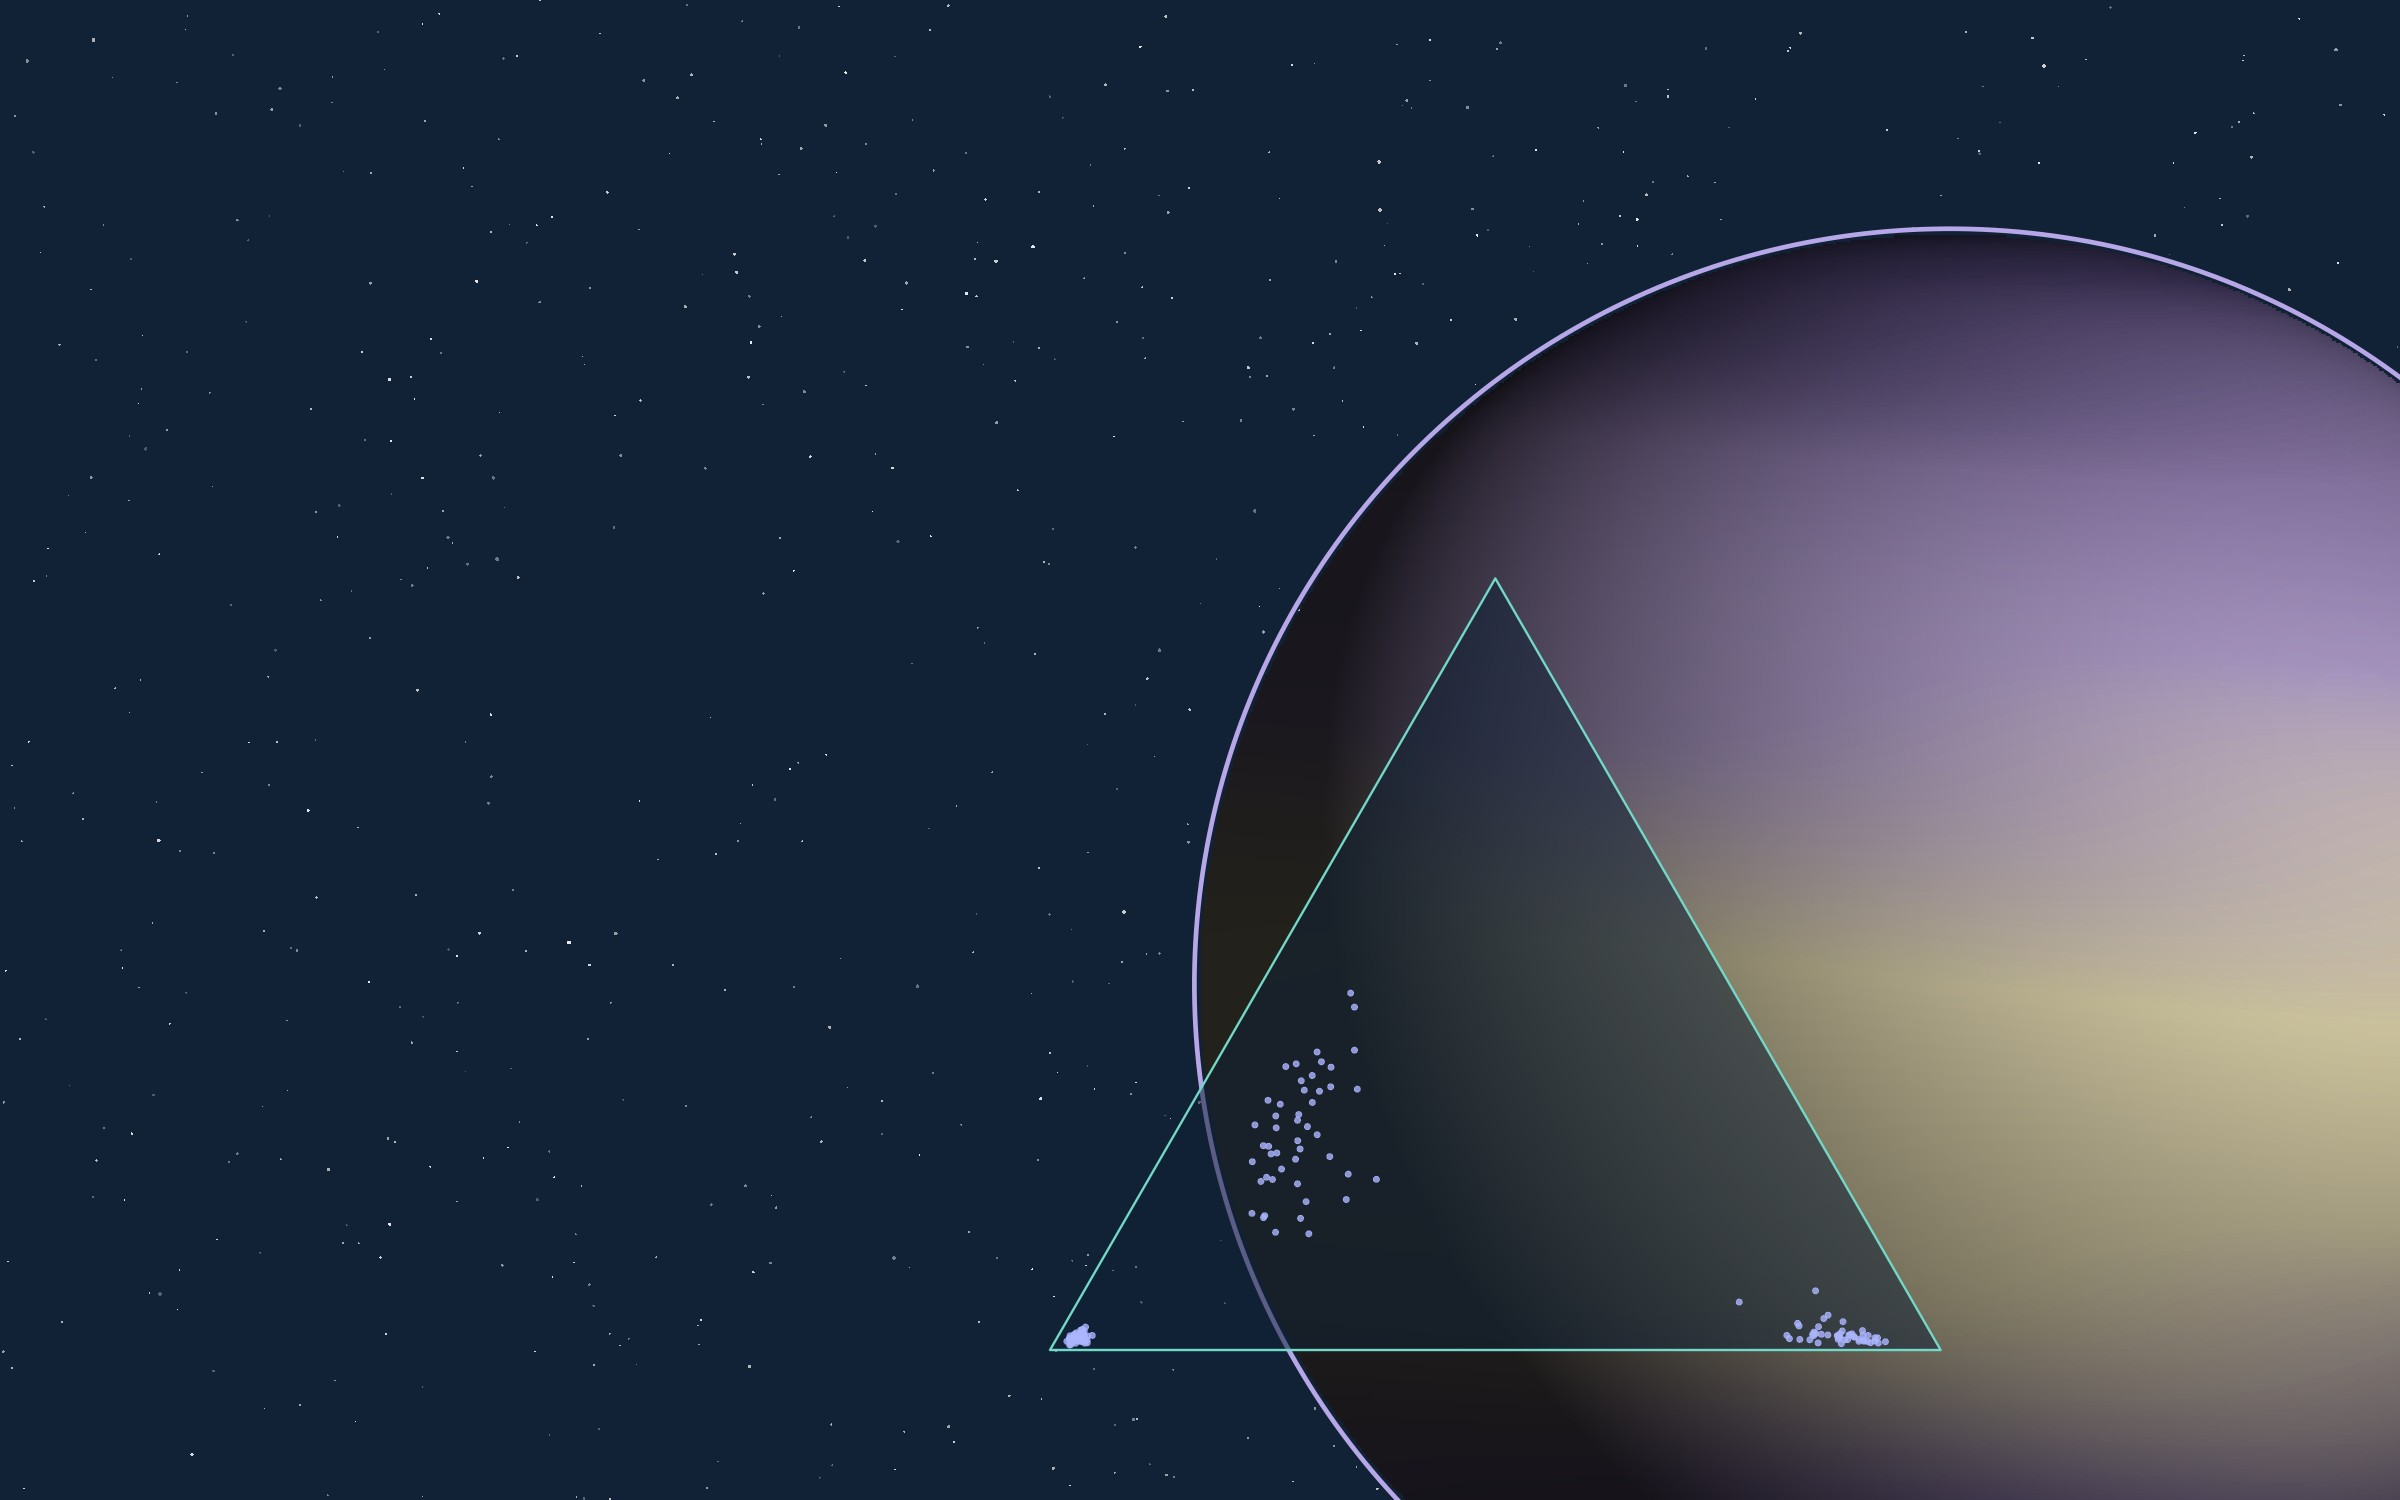
\includegraphics[width=20cm,height=12.5cm]{Scena/copertina.jpg}};}{}
\node[anchor=north west,inner sep=0] at([xshift=1.05cm,yshift=-1.10cm]current page.north west){\color{Mint}\bfseries\fontsize{23}{28}\selectfont SIMPLEX};
\node[anchor=north west,inner sep=0] at([xshift=1.07cm,yshift=-2.16cm]current page.north west){\color{white}\fontsize{9}{12}\selectfont MODULO M17 · SCIENZE DELLA TERRA};
\draw[Mint,line width=1.5pt]([xshift=1.07cm,yshift=-2.78cm]current page.north west)--([xshift=2.6cm,yshift=-2.78cm]current page.north west);
\node[anchor=north west,inner sep=0] at([xshift=1.05cm,yshift=-3.35cm]current page.north west){\begin{minipage}{9.2cm}\raggedright\color{white}\bfseries\fontsize{28.5}{34.5}\selectfont Dati\\composizionali\end{minipage}};
\node[anchor=north west,inner sep=0] at([xshift=1.07cm,yshift=-7.88cm]current page.north west){\begin{minipage}{8.9cm}\raggedright\color{Lilac}\fontsize{12.2}{17}\selectfont Percentuali che sommano a cento\end{minipage}};
\node[anchor=north west,inner sep=0] at([xshift=1.07cm,yshift=-8.70cm]current page.north west){\begin{minipage}{8.9cm}\raggedright\color{white!75}\fontsize{10.3}{14.5}\selectfont Chiusura, log-rapporti e geometria di Aitchison\end{minipage}};
\node[anchor=north west,inner sep=0] at([xshift=1.07cm,yshift=-10.52cm]current page.north west){\color{white}\fontsize{10.5}{14}\selectfont GeoStat Lab · corso di Marzio De Corato};
\node[anchor=north west,inner sep=0] at([xshift=1.07cm,yshift=-11.17cm]current page.north west){\color{Mint}\fontsize{8.8}{11}\selectfont\href{https://creativecommons.org/licenses/by-nc-sa/4.0/}{Impaginazione da Tessera · CC BY-NC-SA 4.0}};
\end{tikzpicture}\end{frame}

\begin{frame}[plain]\hypertarget{slide2}{}
\bookmark[level=1,page=2]{Indice della presentazione}
\begin{tikzpicture}[remember picture,overlay]
\PilotChrome{Indice della presentazione}{PERCORSO}{2}{I titoli dell’indice aprono i capitoli. Il nome del capitolo in alto riporta a questa pagina.}
\node[anchor=north west,inner sep=0] at([xshift=.96cm,yshift=-2.12cm]current page.north west){\Colonna{9.40cm}{\PLabel{Capitoli}
{\fontsize{10.7}{13.5}\selectfont\hyperlink{slide4}{La chiusura e i suoi effetti\hfill 4}\par}\vspace{.16cm}
{\fontsize{10.7}{13.5}\selectfont\hyperlink{slide11}{Rapporti logaritmici\hfill 11}\par}\vspace{.16cm}
{\fontsize{10.7}{13.5}\selectfont\hyperlink{slide18}{Descrivere un insieme di composizioni\hfill 18}\par}\vspace{.16cm}
{\fontsize{10.7}{13.5}\selectfont\hyperlink{slide24}{Zeri, limiti di rivelabilità e modelli\hfill 24}\par}\vspace{.16cm}
}};
\node[anchor=north west,inner sep=0] at([xshift=10.85cm,yshift=-2.12cm]current page.north west){\Colonna{8.16cm}{\PLabel{Percorso di lettura}
\PBody{Centoquarantaquattro analisi sintetiche di diciotto stazioni riportano sei parti in percentuale in massa. Il percorso parte dagli effetti della somma costante, introduce i log-rapporti, descrive centri e variabilità e chiude con i valori sotto il limite di rivelabilità e con un modello per la densità.}
\PInfo{Le pagine Scenario A e Confronto riprendono gli esperimenti nel browser. I valori di partenza del simulatore possono differire dal caso guida.}
\href{https://marzione00.github.io/Lab_Geo/\#modulo-M17}{\color{Classical}\bfseries Apri gli esperimenti di Simplex}}};
\end{tikzpicture}\end{frame}

\begin{frame}[plain]\hypertarget{slide3}{}
\bookmark[level=1,page=3]{La correlazione di −0,92 fra SiO$_2$ e CaO descrive la geochimica o la somma a cento?}
\begin{tikzpicture}[remember picture,overlay]
\PilotChrome{{\fontsize{15.3}{19}\selectfont La correlazione di −0,92 fra SiO$_2$ e CaO descrive la geochimica o la somma a cento?}}{IL CASO GUIDA}{3}{Una percentuale è una parte di un intero: il suo significato dipende dalle altre parti.}
\node[anchor=north west,inner sep=0] at([xshift=.96cm,yshift=-2.12cm]current page.north west){\Colonna{9.40cm}{{\centering\resizebox{.97\linewidth}{!}{\begin{tikzpicture}[x=1cm,y=1cm,every node/.append style={anchor=center,inner sep=.3333em}]
\foreach \x/\n/\t/\col in {0.9/1/Chiusura/GeoA,3.0/2/Log-rapporti/GeoC,5.1/3/Centri/GeoA,7.2/4/Zeri e modelli/GeoB}{
 \draw[\col,fill=\col!8,rounded corners=4pt,line width=.8pt] (\x-.95,1.25) rectangle(\x+.95,3.35);
 \node[font=\bfseries\fontsize{15}{18}\selectfont,text=\col] at(\x,2.75){\n};
 \node[pNote,text width=1.75cm] at(\x,1.85){\t};}
\foreach \x in {1.85,3.95,6.05}{\draw[pEdge] (\x,2.3)--(\x+.2,2.3);}
\draw[Rule,line width=.6pt] (0,.75)--(8.15,.75);
\node[pNote] at(4.08,.35){Percentuali che sommano a cento: che cosa si può confrontare.};
\end{tikzpicture}
}\par}
}};
\node[anchor=north west,inner sep=0] at([xshift=10.85cm,yshift=-2.12cm]current page.north west){\Colonna{8.16cm}{\PLabel{Il caso}
\PBody{Centoquarantaquattro campioni sintetici di arenaria, basalto e calcare, otto per ciascuna di diciotto stazioni, riportano SiO$_2$, Al$_2$O$_3$, CaO, MgO, FeO e una parte residua in percentuale in massa, con somma cento. Quindici campioni hanno una parte sotto il limite di rivelabilità di 0,1\%, registrata come zero.}
\PInfo{Seguiremo i dati dalla chiusura ai log-rapporti, ai centri composizionali e alla sostituzione degli zeri, fino a un modello della densità scritto in coordinate di bilancio.}
}};
\end{tikzpicture}\end{frame}

\begin{frame}[plain]\hypertarget{slide4}{}
\bookmark[level=0,page=4]{La chiusura e i suoi effetti}
\bookmark[level=1,page=4]{Che cosa resta se cambia la base di calcolo?}
\begin{tikzpicture}[remember picture,overlay]
\PilotChrome{Che cosa resta se cambia la base di calcolo?}{LA CHIUSURA E I SUOI EFFETTI}{4}{I rapporti fra le parti restano gli stessi quando la composizione viene riferita a un intero diverso.}
\node[anchor=north west,inner sep=0] at([xshift=.96cm,yshift=-2.12cm]current page.north west){\Colonna{9.40cm}{\PLabel{Domanda}
\PBody{Un basalto contiene il 46,7\% di SiO$_2$ e il 10,4\% di CaO. Riferito alla sola frazione dei cinque ossidi, i due valori diventano più grandi. Quale quantità non cambia?}
\vspace{.35cm}\PLabel{Interpretazione}
\PBody{Il rapporto SiO$_2$/CaO vale 4,49 in entrambe le basi. Le percentuali dipendono dall’intero scelto, il rapporto dipende soltanto dalle due parti.}
}};
\node[anchor=north west,inner sep=0] at([xshift=10.85cm,yshift=-2.12cm]current page.north west){\Colonna{8.16cm}{\begin{tcolorbox}[enhanced,arc=1.7mm,boxrule=.6pt,colback=white,colframe=Classical!60!Navy,colbacktitle=Navy,coltitle=white,fonttitle=\bfseries\small,title={R · calcolo riproducibile},left=1.7mm,right=1.3mm,top=1.1mm,bottom=1.1mm,before skip=1mm,after skip=1.0mm]\lstinputlisting[style=GeoR,language=R]{Codice/capitolo-01.R}\end{tcolorbox}
\PLabel{Risultato in R}
\begin{tcolorbox}[colback=GeoTint,colframe=Rule,boxrule=.5pt,arc=1.4mm,left=2mm,right=1mm,top=1mm,bottom=1mm]{\fontsize{8.6}{11.4}\selectfont\ttfamily \mbox{\ \ intera\ silicati}\\\mbox{\ \ \ \ 4.49\ \ \ \ \ 4.49}}\end{tcolorbox}}};
\end{tikzpicture}\end{frame}

\begin{frame}[plain]\hypertarget{slide5}{}
\bookmark[level=1,page=5]{Il simplesso è lo spazio delle composizioni}
\begin{tikzpicture}[remember picture,overlay]
\PilotChrome{Il simplesso è lo spazio delle composizioni}{LA CHIUSURA E I SUOI EFFETTI}{5}{Una composizione a $D$ parti ha $D-1$ gradi di libertà: l’ultima parte è determinata dalle altre.}
\node[anchor=north west,inner sep=0] at([xshift=.96cm,yshift=-2.12cm]current page.north west){\Colonna{9.40cm}{{\centering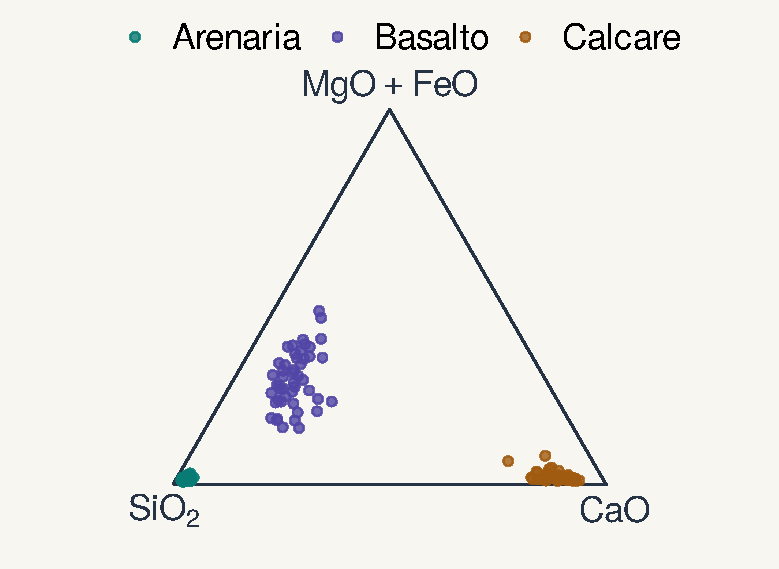
\includegraphics[width=\linewidth,height=6.15cm,keepaspectratio]{Figure/F01.pdf}\par}
\PSmall{Sottocomposizione SiO$_2$, CaO, MgO+FeO chiusa a cento, dopo la sostituzione degli zeri.}
}};
\node[anchor=north west,inner sep=0] at([xshift=10.85cm,yshift=-2.12cm]current page.north west){\Colonna{8.16cm}{\PBody{Una composizione a $D$ parti è un vettore di numeri positivi con somma costante $\kappa$, qui cento. L’insieme di questi vettori è il simplesso. Il diagramma ternario rappresenta una sottocomposizione a tre parti: ogni vertice corrisponde a una parte pura e la distanza da un lato misura la quota della parte opposta. Le arenarie si raccolgono vicino al vertice della silice, i calcari vicino a quello del calcio, i basalti all’interno.}
\par\smallskip{\centering\adjustbox{max width=.98\linewidth}{$\displaystyle \mathcal S^D=\Big\{x\in\mathbb R^D:\ x_i>0,\ \sum_{i=1}^D x_i=\kappa\Big\}$}\par\smallskip}
}};
\end{tikzpicture}\end{frame}

\begin{frame}[plain]\hypertarget{slide6}{}
\bookmark[level=1,page=6]{La somma costante impone covarianze negative}
\begin{tikzpicture}[remember picture,overlay]
\PilotChrome{La somma costante impone covarianze negative}{LA CHIUSURA E I SUOI EFFETTI}{6}{In dati chiusi una parte non può crescere senza che le altre, insieme, diminuiscano.}
\node[anchor=north west,inner sep=0] at([xshift=.96cm,yshift=-2.12cm]current page.north west){\Colonna{9.40cm}{{\centering\resizebox{0.94\linewidth}{!}{\begin{tikzpicture}[x=1cm,y=1cm]
\foreach \y/\a/\b/\c/\n in {3.2/4.0/2.4/1.6/A,1.6/5.2/1.68/1.12/B}{
 \fill[GeoA!70] (0,\y) rectangle (\a,\y+.62);
 \fill[GeoC!60] (\a,\y) rectangle (\a+\b,\y+.62);
 \fill[GeoB!65] (\a+\b,\y) rectangle (\a+\b+\c,\y+.62);
 \draw[Ink,line width=.5pt] (0,\y) rectangle (8,\y+.62);
 \node[pNote,anchor=east] at(-.12,\y+.31){\n};
 \node[pNote,anchor=west] at(8.1,\y+.31){100};}
\node[pLabel,text=white] at(2.0,3.51){$x_1=50$};
\node[pLabel,text=white] at(2.6,1.91){$x_1=65$};
\node[pLabel] at(5.2,3.51){30};\node[pLabel] at(7.2,3.51){20};
\node[pLabel] at(6.04,1.91){21};\node[pLabel] at(7.44,1.91){14};
\draw[pEdge] (4,3.1)--(5.2,2.32);
\node[pNote,text width=7.4cm] at(4,.75){Se $x_1$ cresce, le altre parti devono diminuire insieme:\\le covarianze con $x_1$ sommano a $-\operatorname{var}(x_1)$.};
\end{tikzpicture}
}\par}
\PSmall{Composizione a tre parti prima e dopo l’aumento della prima parte.}
}};
\node[anchor=north west,inner sep=0] at([xshift=10.85cm,yshift=-2.12cm]current page.north west){\Colonna{8.16cm}{\PBody{Poiché la somma delle parti è costante, la sua covarianza con qualunque parte è nulla. Ne segue l’identità osservata da Felix Chayes nel 1960: la somma delle covarianze di una parte con tutte le altre è uguale all’opposto della sua varianza. Nei campioni completi del caso la varianza di SiO$_2$ è 993 e la somma delle sue cinque covarianze vale $-993$. Almeno una covarianza deve quindi essere negativa, qualunque sia la geochimica.}
\par\smallskip{\centering\adjustbox{max width=.98\linewidth}{$\displaystyle \sum_{j\ne i}\operatorname{cov}(x_i,x_j)=-\operatorname{var}(x_i)$}\par\smallskip}
\PSmall{$x_i$ e $x_j$ sono due parti della composizione chiusa; la relazione vale per ogni parte $i$.}
}};
\end{tikzpicture}\end{frame}

\begin{frame}[plain]\hypertarget{slide7}{}
\bookmark[level=1,page=7]{Le correlazioni cambiano con la sottocomposizione}
\begin{tikzpicture}[remember picture,overlay]
\PilotChrome{Le correlazioni cambiano con la sottocomposizione}{LA CHIUSURA E I SUOI EFFETTI}{7}{Un log-rapporto fra due parti è lo stesso in ogni sottocomposizione che le contiene.}
\node[anchor=north west,inner sep=0] at([xshift=.96cm,yshift=-2.12cm]current page.north west){\Colonna{9.40cm}{\PLabel{Domanda}
\PBody{Nei basalti, MgO e FeO sono correlati positivamente o negativamente? La risposta può dipendere da quali altre parti vengono incluse nell’intero?}
\vspace{.35cm}\PLabel{Interpretazione}
\PBody{La correlazione vale 0,373 nella composizione a sei parti e $-0{,}177$ nella sottocomposizione CaO, MgO, FeO. La varianza di $\log(\mathrm{MgO}/\mathrm{FeO})$ resta 0,175 nei due casi.}
}};
\node[anchor=north west,inner sep=0] at([xshift=10.85cm,yshift=-2.12cm]current page.north west){\Colonna{8.16cm}{\begin{tcolorbox}[enhanced,arc=1.7mm,boxrule=.6pt,colback=white,colframe=Classical!60!Navy,colbacktitle=Navy,coltitle=white,fonttitle=\bfseries\small,title={R · calcolo riproducibile},left=1.7mm,right=1.3mm,top=1.1mm,bottom=1.1mm,before skip=1mm,after skip=1.0mm]\lstinputlisting[style=GeoR,language=R]{Codice/capitolo-02.R}\end{tcolorbox}
\PLabel{Risultato in R}
\begin{tcolorbox}[colback=GeoTint,colframe=Rule,boxrule=.5pt,arc=1.4mm,left=2mm,right=1mm,top=1mm,bottom=1mm]{\fontsize{8.6}{11.4}\selectfont\ttfamily \mbox{[1]\ \ 0.373\ -0.177\ \ 0.175\ \ 0.175}}\end{tcolorbox}}};
\end{tikzpicture}\end{frame}

\begin{frame}[plain]\hypertarget{slide8}{}
\bookmark[level=1,page=8]{Parti indipendenti diventano correlate}
\begin{tikzpicture}[remember picture,overlay]
\PilotChrome{Parti indipendenti diventano correlate}{LA CHIUSURA E I SUOI EFFETTI}{8}{Una correlazione fra percentuali va confrontata con quella che la sola chiusura produrrebbe.}
\node[anchor=north west,inner sep=0] at([xshift=.96cm,yshift=-2.12cm]current page.north west){\Colonna{9.40cm}{{\centering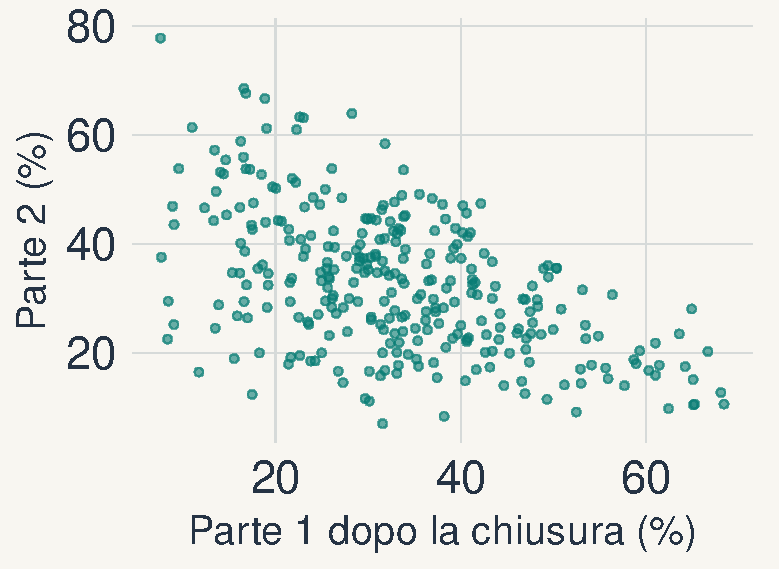
\includegraphics[width=\linewidth,height=6.15cm,keepaspectratio]{Figure/F02.pdf}\par}
\PSmall{Trecento composizioni simulate da tre parti lognormali indipendenti, chiuse a cento.}
}};
\node[anchor=north west,inner sep=0] at([xshift=10.85cm,yshift=-2.12cm]current page.north west){\Colonna{8.16cm}{\PBody{Karl Pearson descrisse nel 1897 la correlazione spuria che nasce fra indici con lo stesso denominatore. Nella simulazione tre parti indipendenti hanno correlazione 0,045 fra le prime due; dopo la chiusura la stessa coppia ha correlazione $-0{,}519$. Quando le parti hanno la stessa varianza e le stesse covarianze, il vincolo di Chayes fissa la correlazione media fra coppie al valore riportato sotto.}
\par\smallskip{\centering\adjustbox{max width=.98\linewidth}{$\displaystyle \bar r=-\frac{1}{D-1}$}\par\smallskip}
\PSmall{$D$ è il numero delle parti; con tre parti il valore è $-0{,}5$, con dieci parti $-0{,}11$.}
}};
\end{tikzpicture}\end{frame}

\begin{frame}[plain]\hypertarget{slide9}{}
\bookmark[level=1,page=9]{Chiusura e correlazione spuria}
\begin{tikzpicture}[remember picture,overlay]
\PilotChrome{Chiusura e correlazione spuria}{LA CHIUSURA E I SUOI EFFETTI}{9}{Osservare le correlazioni che la chiusura a cento introduce fra parti generate indipendenti.}
\node[anchor=north west,inner sep=0] at([xshift=.96cm,yshift=-2.12cm]current page.north west){\Colonna{9.40cm}{{\centering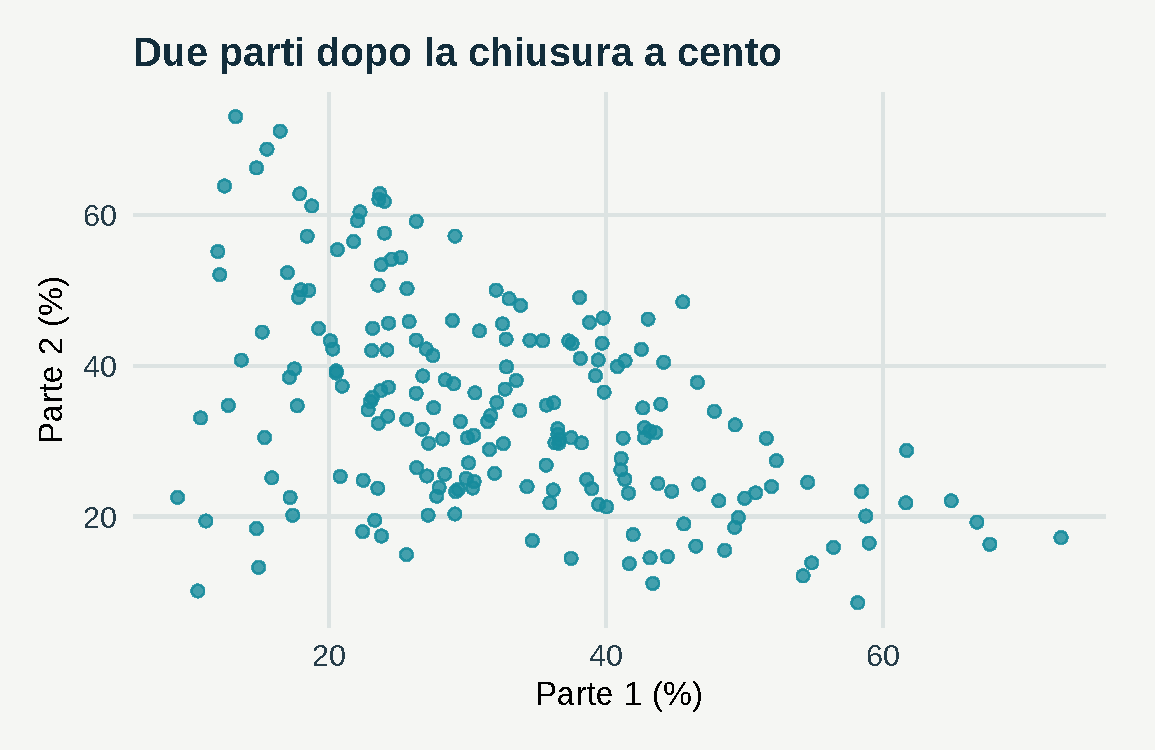
\includegraphics[width=\linewidth,height=6.0cm,keepaspectratio]{Esperimenti/m17-chiusura-A.pdf}\par}
\PSmall{Numero delle parti: 3. Seme: 17.}
}};
\node[anchor=north west,inner sep=0] at([xshift=10.85cm,yshift=-2.12cm]current page.north west){\Colonna{8.16cm}{\PLabel{Scenario A · simulazione}
\PBody{L’esperimento genera duecento campioni con $D$ parti lognormali indipendenti e con la stessa dispersione, poi li chiude a cento. Confronta la correlazione media fra le coppie di parti prima e dopo la chiusura con il valore imposto dal vincolo.}
\par\smallskip{\centering\adjustbox{max width=.98\linewidth}{$\displaystyle \sum_{j\ne i}\operatorname{cov}(x_i,x_j)=-\operatorname{var}(x_i)$}\par\smallskip}
\PSmall{$D$ parti scambiabili: la correlazione media dopo la chiusura tende a $-1/(D-1)$.}
}};
\node[anchor=north east,inner sep=0] at([xshift=17.1cm,yshift=-12.04cm]current page.north west){\fontsize{7.7}{9}\selectfont \href{https://marzione00.github.io/Lab_Geo/\#laboratorio/m17-chiusura}{\color{Classical}\bfseries Apri il laboratorio · m17-chiusura}};
\end{tikzpicture}\end{frame}

\begin{frame}[plain]\hypertarget{slide10}{}
\bookmark[level=1,page=10]{Confronto | Chiusura e correlazione spuria}
\begin{tikzpicture}[remember picture,overlay]
\PilotChrome{Confronto | Chiusura e correlazione spuria}{LA CHIUSURA E I SUOI EFFETTI}{10}{La chiusura produce correlazioni negative anche fra parti indipendenti; la loro entità dipende da $D$.}
\node[anchor=north west,inner sep=0] at([xshift=.96cm,yshift=-2.12cm]current page.north west){\Colonna{9.40cm}{{\centering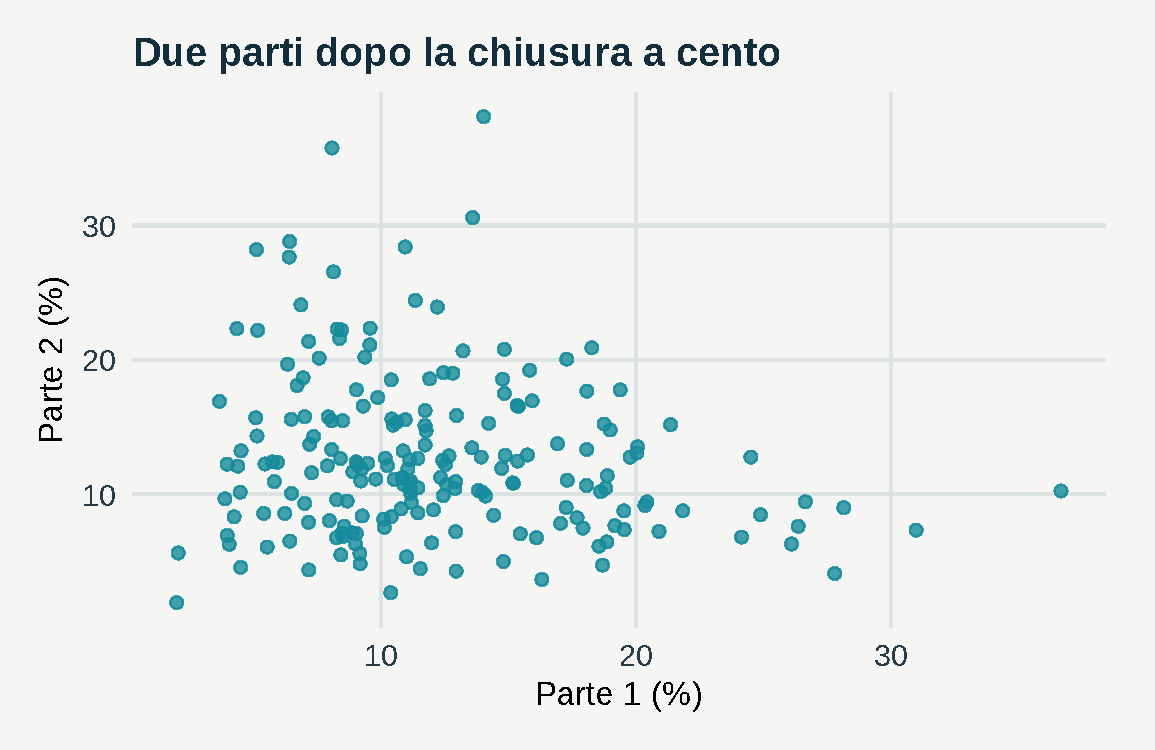
\includegraphics[width=\linewidth,height=5.6cm,keepaspectratio]{Esperimenti/m17-chiusura-B.pdf}\par}
\PSmall{Numero delle parti: 3 $\to$ 8. Tutti gli altri parametri e il seme sono fissi.}
}};
\node[anchor=north west,inner sep=0] at([xshift=10.85cm,yshift=-2.12cm]current page.north west){\Colonna{8.16cm}{\PLabel{Confronto fra gli scenari}
{\fontsize{10.2}{12.8}\selectfont\begin{tabular}{@{}>{\raggedright\arraybackslash}p{0.48\linewidth}@{\hspace{.13cm}}>{\raggedright\arraybackslash}p{0.224\linewidth}@{\hspace{.13cm}}>{\raggedright\arraybackslash}p{0.224\linewidth}@{}}\toprule Grandezza & A & B\\[2.3pt]
\midrule 
Correlazione media prima & 0{,}0506 & -0{,}0115\\[2.3pt]
Correlazione media dopo & -0{,}499 & -0{,}142\\[2.3pt]
Valore $-1/(D-1)$ & -0{,}5 & -0{,}143\\[2.3pt]
Coppie di parti & 3 & 28\\[2.3pt]
\bottomrule\end{tabular}\par}
\vspace{.25cm}\PBody{Con otto parti il vincolo si distribuisce su ventotto coppie e la correlazione media dopo la chiusura scende in valore assoluto da circa 0,50 a 0,14. Prima della chiusura le medie restano vicine a zero.}
}};
\node[anchor=north east,inner sep=0] at([xshift=17.1cm,yshift=-12.04cm]current page.north west){\fontsize{7.7}{9}\selectfont \href{https://marzione00.github.io/Lab_Geo/\#laboratorio/m17-chiusura}{\color{Classical}\bfseries Apri il laboratorio · m17-chiusura}};
\end{tikzpicture}\end{frame}

\begin{frame}[plain]\hypertarget{slide11}{}
\bookmark[level=0,page=11]{Rapporti logaritmici}
\bookmark[level=1,page=11]{Il log-rapporto non dipende dalla chiusura}
\begin{tikzpicture}[remember picture,overlay]
\PilotChrome{Il log-rapporto non dipende dalla chiusura}{RAPPORTI LOGARITMICI}{11}{I log-rapporti sono invarianti di scala, simmetrici e additivi lungo una catena di parti.}
\node[anchor=north west,inner sep=0] at([xshift=.96cm,yshift=-2.12cm]current page.north west){\Colonna{9.40cm}{{\centering\resizebox{0.94\linewidth}{!}{\begin{tikzpicture}[x=1cm,y=1cm]
\node[pFlow,minimum width=1.7cm] (a) at(0,0){$x_a$};
\node[pFlow,minimum width=1.7cm] (b) at(6,0){$x_b$};
\node[pFlow,minimum width=1.7cm] (c) at(3,3.6){$x_c$};
\draw[pEdge] (a)--node[pLabel,below]{$\log(x_b/x_a)$}(b);
\draw[pEdge] (b)--node[pLabel,right,xshift=2mm]{$\log(x_c/x_b)$}(c);
\draw[pEdge] (a)--node[pLabel,left,xshift=-2mm]{$\log(x_c/x_a)$}(c);
\node[pNote,text width=7.6cm] at(3,-1.55){$\log\frac{x_c}{x_a}=\log\frac{x_b}{x_a}+\log\frac{x_c}{x_b}$.\\ Moltiplicare tutte le parti per $\lambda>0$ non cambia nessun lato.};
\end{tikzpicture}
}\par}
\PSmall{Tre parti e i loro log-rapporti.}
}};
\node[anchor=north west,inner sep=0] at([xshift=10.85cm,yshift=-2.12cm]current page.north west){\Colonna{8.16cm}{\PBody{John Aitchison propose nel 1982 di analizzare le composizioni attraverso i logaritmi dei rapporti fra le parti. Un log-rapporto non cambia se tutte le parti vengono moltiplicate per la stessa costante, per cui è lo stesso nei dati grezzi, in quelli chiusi a cento e in ogni sottocomposizione. Scambiare le parti cambia soltanto il segno, e i log-rapporti si sommano lungo una catena.}
\par\smallskip{\centering\adjustbox{max width=.98\linewidth}{$\displaystyle \log\frac{\lambda x_i}{\lambda x_j}=\log\frac{x_i}{x_j},\qquad \lambda>0$}\par\smallskip}
}};
\end{tikzpicture}\end{frame}

\begin{frame}[plain]\hypertarget{slide12}{}
\bookmark[level=1,page=12]{Due trasformazioni dei log-rapporti}
\begin{tikzpicture}[remember picture,overlay]
\PilotChrome{Due trasformazioni dei log-rapporti}{RAPPORTI LOGARITMICI}{12}{La trasformazione alr dipende dalla parte scelta come denominatore; la clr tratta tutte le parti allo stesso modo.}
\node[anchor=north west,inner sep=0] at([xshift=.96cm,yshift=-2.12cm]current page.north west){\Colonna{9.40cm}{\PBody{La trasformazione alr divide le prime $D-1$ parti per l’ultima e ne prende il logaritmo; il risultato cambia con la parte scelta come denominatore. La trasformazione clr divide ogni parte per la media geometrica di tutte le parti. Per lo stesso basalto il codice calcola le due trasformazioni con Altro come denominatore della alr: le coordinate clr sommano a zero.}
\par\smallskip{\centering\adjustbox{max width=.98\linewidth}{$\displaystyle \operatorname{clr}_i(x)=\log\frac{x_i}{g(x)},\qquad g(x)=\Big(\prod_{j=1}^D x_j\Big)^{1/D}$}\par\smallskip}
}};
\node[anchor=north west,inner sep=0] at([xshift=10.85cm,yshift=-2.12cm]current page.north west){\Colonna{8.16cm}{\begin{tcolorbox}[enhanced,arc=1.7mm,boxrule=.6pt,colback=white,colframe=Classical!60!Navy,colbacktitle=Navy,coltitle=white,fonttitle=\bfseries\small,title={R · calcolo riproducibile},left=1.7mm,right=1.3mm,top=1.1mm,bottom=1.1mm,before skip=1mm,after skip=1.0mm]\lstinputlisting[style=GeoR,language=R]{Codice/capitolo-03.R}\end{tcolorbox}
\PLabel{Risultato in R}
\begin{tcolorbox}[colback=GeoTint,colframe=Rule,boxrule=.5pt,arc=1.4mm,left=2mm,right=1mm,top=1mm,bottom=1mm]{\fontsize{8.6}{11.4}\selectfont\ttfamily \mbox{\ \ \ \ \ SiO2\ Al2O3\ \ \ \ CaO\ \ \ \ MgO\ \ \ FeO\ \ Altro}\\\mbox{alr\ 2.052\ 0.803\ \ 0.550\ \ 0.312\ 0.803\ \ 0.000}\\\mbox{clr\ 1.298\ 0.050\ -0.204\ -0.441\ 0.050\ -0.754}\\\mbox{[1]\ 0}}\end{tcolorbox}}};
\end{tikzpicture}\end{frame}

\begin{frame}[plain]\hypertarget{slide13}{}
\bookmark[level=1,page=13]{Proprietà delle coordinate clr}
\begin{tikzpicture}[remember picture,overlay]
\PilotChrome{Proprietà delle coordinate clr}{RAPPORTI LOGARITMICI}{13}{Le coordinate clr sono vincolate a somma zero: la loro matrice di covarianza è singolare.}
\node[anchor=north west,inner sep=0] at([xshift=.96cm,yshift=-2.12cm]current page.north west){\Colonna{9.40cm}{\PLabel{Geometria}
\PBody{Le operazioni naturali del simplesso sono la perturbazione, prodotto parte per parte seguito dalla chiusura, e la potenza, elevamento di ogni parte allo stesso esponente seguito dalla chiusura. Con queste operazioni il simplesso è uno spazio vettoriale, e la trasformazione clr lo porta in un sottospazio di $\mathbb R^D$ conservando somme e prodotti per uno scalare.}
\par\smallskip{\centering\adjustbox{max width=.98\linewidth}{$\displaystyle x\oplus y=\mathcal C(x_1y_1,\ldots,x_Dy_D),\qquad \alpha\odot x=\mathcal C(x_1^\alpha,\ldots,x_D^\alpha)$}\par\smallskip}
}};
\node[anchor=north west,inner sep=0] at([xshift=10.85cm,yshift=-2.12cm]current page.north west){\Colonna{8.16cm}{\PLabel{Conseguenze per l’analisi}
\PBody{Le coordinate clr sommano a zero, e una qualunque di esse è determinata dalle altre. La loro matrice di covarianza ha quindi determinante nullo e nessuna inversa: i metodi che richiedono l’inversa, come la regressione multipla o la distanza di Mahalanobis, usano $D-1$ coordinate indipendenti. Le varianze delle coordinate clr dipendono dall’insieme completo delle parti.}
\PSmall{$\mathcal C$ indica la chiusura a somma $\kappa$; $\oplus$ è la perturbazione, $\odot$ la potenza.}
}};
\end{tikzpicture}\end{frame}

\begin{frame}[plain]\hypertarget{slide14}{}
\bookmark[level=1,page=14]{I bilanci separano gruppi di parti}
\begin{tikzpicture}[remember picture,overlay]
\PilotChrome{I bilanci separano gruppi di parti}{RAPPORTI LOGARITMICI}{14}{Una partizione binaria sequenziale definisce $D-1$ coordinate ortonormali, ciascuna interpretabile.}
\node[anchor=north west,inner sep=0] at([xshift=.96cm,yshift=-2.12cm]current page.north west){\Colonna{9.40cm}{{\centering\resizebox{0.94\linewidth}{!}{\begin{tikzpicture}[x=1cm,y=-1cm,every node/.style={font=\sffamily\fontsize{10.5}{13}\selectfont,text=Ink,anchor=center,inner sep=.3333em}]
\node[pFlow,minimum width=7.6cm] (r) at(3.9,0){SiO$_2$ \ Al$_2$O$_3$ \ CaO \ MgO \ FeO \ Altro};
\node[pFlow,minimum width=3.0cm,draw=GeoB] (k) at(1.5,1.6){CaO \ Altro};
\node[pFlow,minimum width=4.2cm,draw=GeoA] (s) at(5.6,1.6){SiO$_2$ \ Al$_2$O$_3$ \ MgO \ FeO};
\node[pFlow,minimum width=1.2cm] (k1) at(.8,3.2){CaO}; \node[pFlow,minimum width=1.2cm] (k2) at(2.3,3.2){Altro};
\node[pFlow,minimum width=2.0cm] (s1) at(4.4,3.2){SiO$_2$ \ Al$_2$O$_3$}; \node[pFlow,minimum width=2.0cm] (s2) at(6.9,3.2){MgO \ FeO};
\draw[pEdge] (r)--node[pNote,left]{$b_1$}(k); \draw[pEdge] (r)--(s);
\draw[pEdge] (k)--node[pNote,left]{$b_2$}(k1); \draw[pEdge] (k)--(k2);
\draw[pEdge] (s)--node[pNote,left]{$b_3$}(s1); \draw[pEdge] (s)--(s2);
\node[pNote] at(4.4,4.25){$b_4$: SiO$_2$ | Al$_2$O$_3$}; \node[pNote] at(6.9,4.25){$b_5$: MgO | FeO};
\end{tikzpicture}
}\par}
\PSmall{Partizione binaria sequenziale delle sei parti e i primi tre bilanci.}
}};
\node[anchor=north west,inner sep=0] at([xshift=10.85cm,yshift=-2.12cm]current page.north west){\Colonna{8.16cm}{\PBody{Juan José Egozcue e colleghi introdussero nel 2003 le trasformazioni isometriche, che forniscono $D-1$ coordinate ortonormali; nel 2005 Egozcue e Vera Pawlowsky-Glahn le costruirono con una partizione binaria sequenziale, che divide le parti in due gruppi e poi ogni gruppo in due, fino a parti singole. Ogni divisione produce un bilancio, il log-rapporto fra le medie geometriche dei due gruppi con un fattore di normalizzazione.}
\par\smallskip{\centering\adjustbox{max width=.98\linewidth}{$\displaystyle b=\sqrt{\frac{rs}{r+s}}\,\log\frac{g(x_+)}{g(x_-)}$}\par\smallskip}
\PSmall{$x_+$ e $x_-$ sono i due gruppi di parti, con $r$ e $s$ parti; $g$ è la media geometrica.}
}};
\end{tikzpicture}\end{frame}

\begin{frame}[plain]\hypertarget{slide15}{}
\bookmark[level=1,page=15]{Lo stesso spostamento pesa in modo diverso}
\begin{tikzpicture}[remember picture,overlay]
\PilotChrome{Lo stesso spostamento pesa in modo diverso}{RAPPORTI LOGARITMICI}{15}{La distanza di Aitchison misura variazioni relative delle parti.}
\node[anchor=north west,inner sep=0] at([xshift=.96cm,yshift=-2.12cm]current page.north west){\Colonna{9.40cm}{\PBody{La distanza di Aitchison è la distanza euclidea fra le coordinate clr. Nel codice due coppie di composizioni differiscono per 0,1 punti percentuali spostati fra due parti, con la stessa distanza euclidea di 0,141. Nella prima coppia MgO passa da 0,1 a 0,2 e raddoppia; nella seconda SiO$_2$ passa da 50 a 50,1. Le distanze di Aitchison valgono 0,633 e 0,005.}
\par\smallskip{\centering\adjustbox{max width=.98\linewidth}{$\displaystyle d_A(x,y)=\big\lVert\operatorname{clr}(x)-\operatorname{clr}(y)\big\rVert$}\par\smallskip}
}};
\node[anchor=north west,inner sep=0] at([xshift=10.85cm,yshift=-2.12cm]current page.north west){\Colonna{8.16cm}{\begin{tcolorbox}[enhanced,arc=1.7mm,boxrule=.6pt,colback=white,colframe=Classical!60!Navy,colbacktitle=Navy,coltitle=white,fonttitle=\bfseries\small,title={R · calcolo riproducibile},left=1.7mm,right=1.3mm,top=1.1mm,bottom=1.1mm,before skip=1mm,after skip=1.0mm]\lstinputlisting[style=GeoR,language=R]{Codice/capitolo-04.R}\end{tcolorbox}
\PLabel{Risultato in R}
\begin{tcolorbox}[colback=GeoTint,colframe=Rule,boxrule=.5pt,arc=1.4mm,left=2mm,right=1mm,top=1mm,bottom=1mm]{\fontsize{8.6}{11.4}\selectfont\ttfamily \mbox{\ \ \ eu\ ait\_a\ ait\_c}\\\mbox{0.141\ 0.633\ 0.005}}\end{tcolorbox}}};
\end{tikzpicture}\end{frame}

\begin{frame}[plain]\hypertarget{slide16}{}
\bookmark[level=1,page=16]{Distanza euclidea e distanza di Aitchison}
\begin{tikzpicture}[remember picture,overlay]
\PilotChrome{Distanza euclidea e distanza di Aitchison}{RAPPORTI LOGARITMICI}{16}{Confrontare l’effetto dello stesso spostamento assoluto su una parte minore e su una parte maggiore.}
\node[anchor=north west,inner sep=0] at([xshift=.96cm,yshift=-2.12cm]current page.north west){\Colonna{9.40cm}{{\centering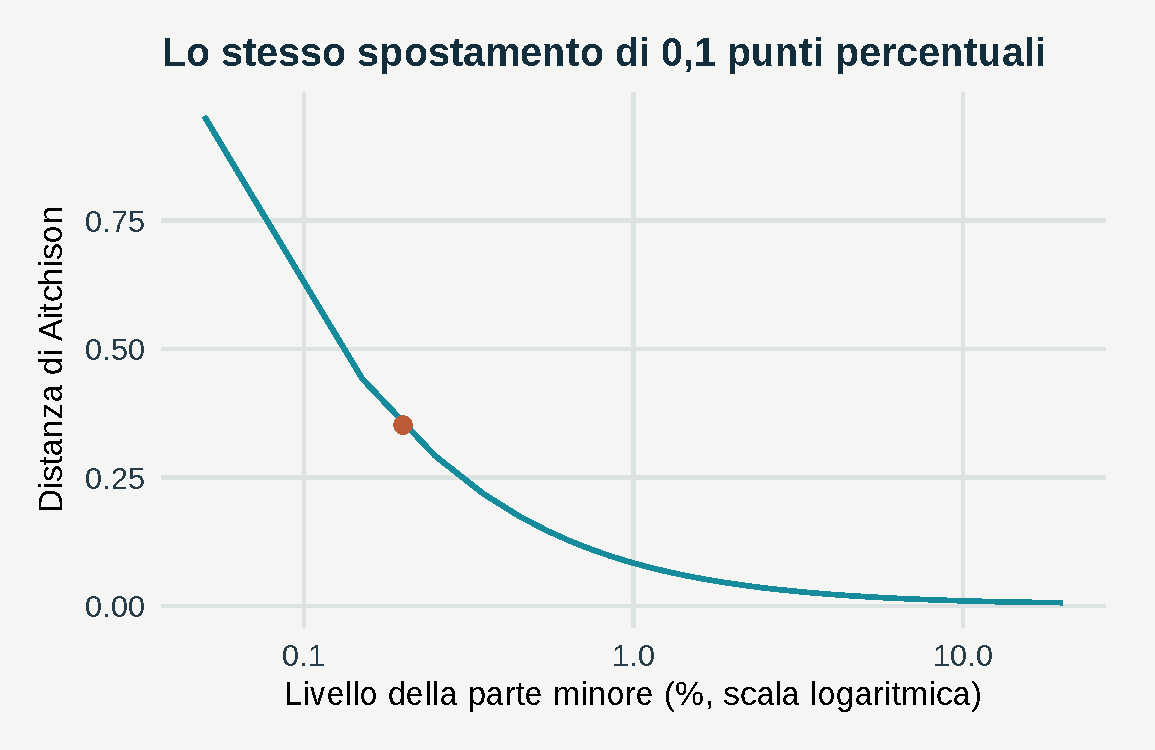
\includegraphics[width=\linewidth,height=6.0cm,keepaspectratio]{Esperimenti/m17-distanze-A.pdf}\par}
\PSmall{Livello della parte minore: 0,2\%. Seme: 17.}
}};
\node[anchor=north west,inner sep=0] at([xshift=10.85cm,yshift=-2.12cm]current page.north west){\Colonna{8.16cm}{\PLabel{Scenario A · simulazione}
\PBody{Due composizioni a quattro parti differiscono per 0,1 punti percentuali spostati dalla parte maggiore alla parte minore. La distanza euclidea resta costante; la curva riporta la distanza di Aitchison per livelli della parte minore fra 0,05 e 20\%.}
\par\smallskip{\centering\adjustbox{max width=.98\linewidth}{$\displaystyle d_A(x,y)=\Big[\sum_{i=1}^D\big(\operatorname{clr}_i(x)-\operatorname{clr}_i(y)\big)^2\Big]^{1/2}$}\par\smallskip}
\PSmall{Il calcolo è deterministico: il seme non cambia il risultato.}
}};
\node[anchor=north east,inner sep=0] at([xshift=17.1cm,yshift=-12.04cm]current page.north west){\fontsize{7.7}{9}\selectfont \href{https://marzione00.github.io/Lab_Geo/\#laboratorio/m17-distanze}{\color{Classical}\bfseries Apri il laboratorio · m17-distanze}};
\end{tikzpicture}\end{frame}

\begin{frame}[plain]\hypertarget{slide17}{}
\bookmark[level=1,page=17]{Confronto | Distanza euclidea e distanza di Aitchison}
\begin{tikzpicture}[remember picture,overlay]
\PilotChrome{{\fontsize{15.3}{19}\selectfont Confronto | Distanza euclidea e distanza di Aitchison}}{RAPPORTI LOGARITMICI}{17}{Lo stesso spostamento in punti percentuali pesa molto di più su una parte in traccia.}
\node[anchor=north west,inner sep=0] at([xshift=.96cm,yshift=-2.12cm]current page.north west){\Colonna{9.40cm}{{\centering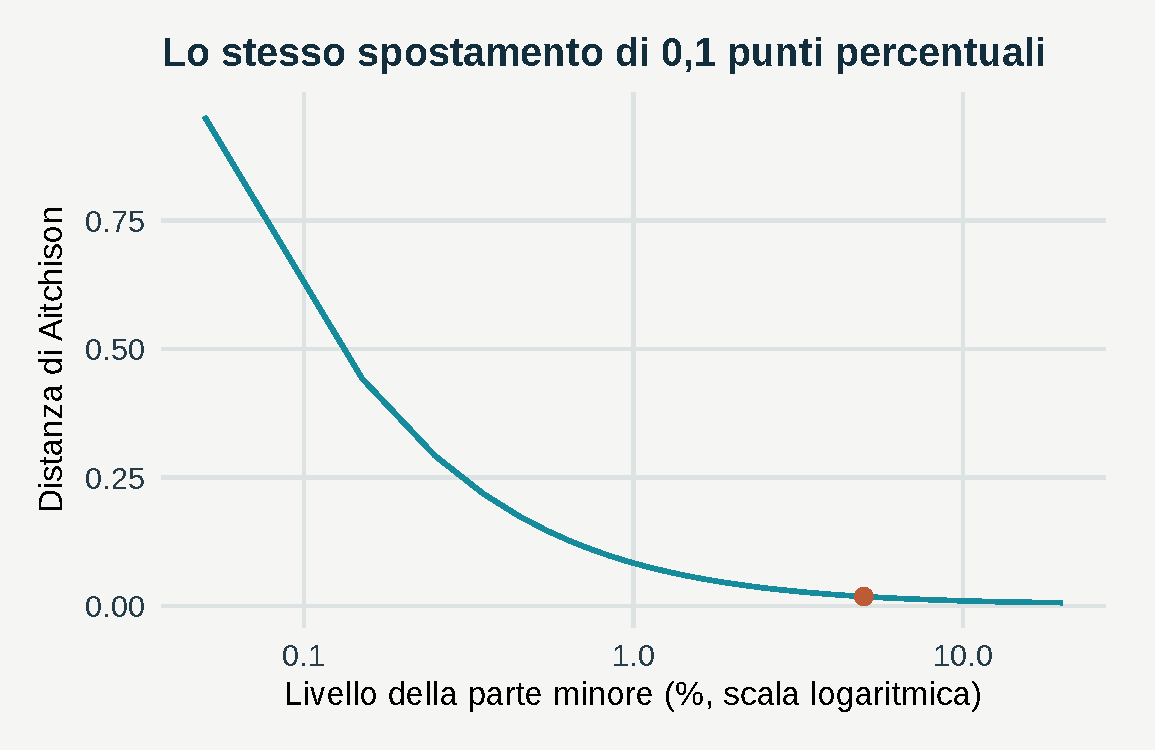
\includegraphics[width=\linewidth,height=5.6cm,keepaspectratio]{Esperimenti/m17-distanze-B.pdf}\par}
\PSmall{Livello della parte minore: 0,2 $\to$ 5\%. Tutti gli altri parametri sono fissi.}
}};
\node[anchor=north west,inner sep=0] at([xshift=10.85cm,yshift=-2.12cm]current page.north west){\Colonna{8.16cm}{\PLabel{Confronto fra gli scenari}
{\fontsize{10.2}{12.8}\selectfont\begin{tabular}{@{}>{\raggedright\arraybackslash}p{0.48\linewidth}@{\hspace{.13cm}}>{\raggedright\arraybackslash}p{0.224\linewidth}@{\hspace{.13cm}}>{\raggedright\arraybackslash}p{0.224\linewidth}@{}}\toprule Grandezza & A & B\\[2.3pt]
\midrule 
Distanza euclidea & 0{,}141 & 0{,}141\\[2.3pt]
Distanza di Aitchison & 0{,}352 & 0{,}0179\\[2.3pt]
Rapporto Aitchison/euclidea & 2{,}49 & 0{,}126\\[2.3pt]
\bottomrule\end{tabular}\par}
\vspace{.25cm}\PBody{Con la parte minore allo 0,2\% lo spostamento ne aumenta la quota della metà e la distanza di Aitchison vale 0,352. Con la parte al 5\% lo stesso spostamento è del 2\% e la distanza scende a 0,018.}
}};
\node[anchor=north east,inner sep=0] at([xshift=17.1cm,yshift=-12.04cm]current page.north west){\fontsize{7.7}{9}\selectfont \href{https://marzione00.github.io/Lab_Geo/\#laboratorio/m17-distanze}{\color{Classical}\bfseries Apri il laboratorio · m17-distanze}};
\end{tikzpicture}\end{frame}

\begin{frame}[plain]\hypertarget{slide18}{}
\bookmark[level=0,page=18]{Descrivere un insieme di composizioni}
\bookmark[level=1,page=18]{Il centro è una media geometrica chiusa}
\begin{tikzpicture}[remember picture,overlay]
\PilotChrome{Il centro è una media geometrica chiusa}{DESCRIVERE UN INSIEME DI COMPOSIZIONI}{18}{Il centro composizionale media i log-rapporti; la media aritmetica media le percentuali.}
\node[anchor=north west,inner sep=0] at([xshift=.96cm,yshift=-2.12cm]current page.north west){\Colonna{9.40cm}{\PBody{Il centro di un insieme di composizioni è la media geometrica di ogni parte, chiusa a cento. Equivale alla media delle coordinate clr riportata nel simplesso. Per i quarantotto basalti la media aritmetica di MgO vale 8,95\% e il centro 8,39\%; per SiO$_2$ i due valori sono 46,37 e 47,25\%. Le parti più disperse in termini relativi mostrano le differenze maggiori.}
\par\smallskip{\centering\adjustbox{max width=.98\linewidth}{$\displaystyle \operatorname{cen}(X)=\mathcal C\big(g_1,\ldots,g_D\big),\quad g_j=\Big(\prod_{k=1}^n x_{kj}\Big)^{1/n}$}\par\smallskip}
}};
\node[anchor=north west,inner sep=0] at([xshift=10.85cm,yshift=-2.12cm]current page.north west){\Colonna{8.16cm}{\begin{tcolorbox}[enhanced,arc=1.7mm,boxrule=.6pt,colback=white,colframe=Classical!60!Navy,colbacktitle=Navy,coltitle=white,fonttitle=\bfseries\small,title={R · calcolo riproducibile},left=1.7mm,right=1.3mm,top=1.1mm,bottom=1.1mm,before skip=1mm,after skip=1.0mm]\lstinputlisting[style=GeoR,language=R]{Codice/capitolo-05.R}\end{tcolorbox}
\PLabel{Risultato in R}
\begin{tcolorbox}[colback=GeoTint,colframe=Rule,boxrule=.5pt,arc=1.4mm,left=2mm,right=1mm,top=1mm,bottom=1mm]{\fontsize{8.6}{11.4}\selectfont\ttfamily \mbox{\ \ \ \ \ \ \ \ \ \ \ \ SiO2\ Al2O3\ \ \ CaO\ \ MgO\ \ \ FeO\ Altro}\\\mbox{aritmetico\ 46.37\ 13.55\ 11.26\ 8.95\ 13.70\ \ 6.16}\\\mbox{geometrico\ 47.25\ 13.64\ 11.10\ 8.39\ 13.43\ \ 6.19}}\end{tcolorbox}}};
\end{tikzpicture}\end{frame}

\begin{frame}[plain]\hypertarget{slide19}{}
\bookmark[level=1,page=19]{La matrice di variazione riassume la dispersione}
\begin{tikzpicture}[remember picture,overlay]
\PilotChrome{La matrice di variazione riassume la dispersione}{DESCRIVERE UN INSIEME DI COMPOSIZIONI}{19}{Una varianza di log-rapporto vicina a zero indica due parti quasi proporzionali.}
\node[anchor=north west,inner sep=0] at([xshift=.96cm,yshift=-2.12cm]current page.north west){\Colonna{9.40cm}{{\centering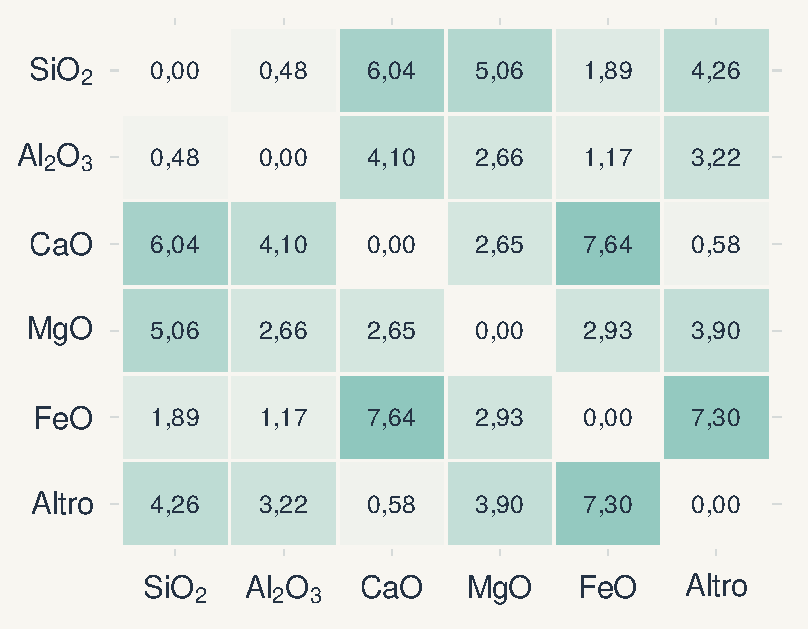
\includegraphics[width=\linewidth,height=6.3cm,keepaspectratio]{Figure/F04.pdf}\par}
\PSmall{Varianze di $\log(x_i/x_j)$ sui 144 campioni, dopo la sostituzione degli zeri.}
}};
\node[anchor=north west,inner sep=0] at([xshift=10.85cm,yshift=-2.12cm]current page.north west){\Colonna{8.16cm}{\PBody{Aitchison descrisse la variabilità con le varianze di tutti i log-rapporti. Un valore vicino a zero indica parti che variano in proporzione: SiO$_2$ e Al$_2$O$_3$ hanno varianza 0,48, CaO e Altro 0,58, perché nei calcari la parte residua contiene soprattutto la CO$_2$ legata al calcio. I valori maggiori, 7,64 per CaO e FeO, separano le litologie. La variabilità totale vale 8,98.}
\par\smallskip{\centering\adjustbox{max width=.98\linewidth}{$\displaystyle \tau_{ij}=\operatorname{var}\Big(\log\frac{x_i}{x_j}\Big),\qquad \operatorname{totvar}=\frac{1}{2D}\sum_{i,j}\tau_{ij}$}\par\smallskip}
}};
\end{tikzpicture}\end{frame}

\begin{frame}[plain]\hypertarget{slide20}{}
\bookmark[level=1,page=20]{Il biplot delle coordinate clr}
\begin{tikzpicture}[remember picture,overlay]
\PilotChrome{Il biplot delle coordinate clr}{DESCRIVERE UN INSIEME DI COMPOSIZIONI}{20}{Il biplot composizionale si costruisce sulle coordinate clr centrate, mai sulle percentuali.}
\node[anchor=north west,inner sep=0] at([xshift=.96cm,yshift=-2.12cm]current page.north west){\Colonna{9.40cm}{{\centering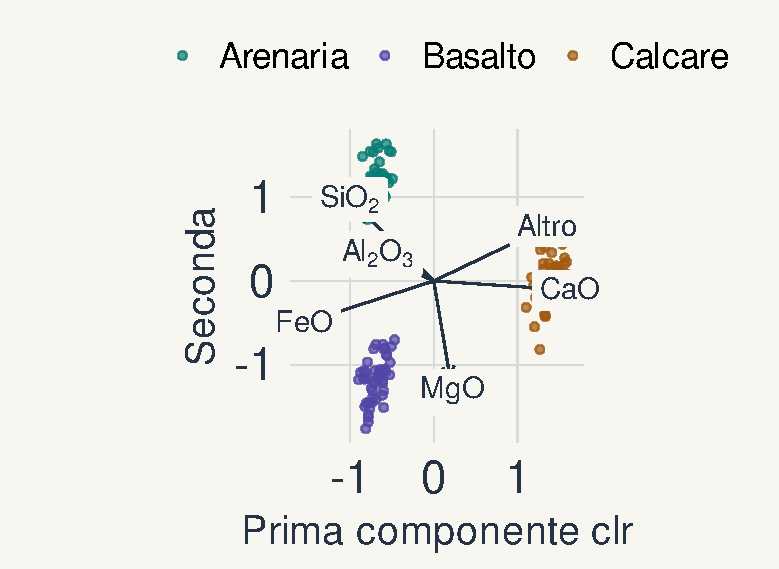
\includegraphics[width=\linewidth,height=6.15cm,keepaspectratio]{Figure/F05.pdf}\par}
\PSmall{Biplot di covarianza delle coordinate clr: punteggi standardizzati, raggi scalati con le deviazioni standard delle componenti.}
}};
\node[anchor=north west,inner sep=0] at([xshift=10.85cm,yshift=-2.12cm]current page.north west){\Colonna{8.16cm}{\PBody{Le componenti principali delle coordinate clr riassumono la variabilità totale. Nel caso la prima componente ne spiega il 69,4\% e la seconda il 28,9\%: i tre gruppi di campioni occupano regioni separate, e i raggi indicano le parti che li distinguono. I raggi di SiO$_2$ e Al$_2$O$_3$ quasi coincidono, coerenti con la piccola varianza del loro log-rapporto.}
\PSmall{Le quote si riferiscono all’insieme delle tre litologie: la dispersione è dominata dalle differenze fra i gruppi.}
}};
\end{tikzpicture}\end{frame}

\begin{frame}[plain]\hypertarget{slide21}{}
\bookmark[level=1,page=21]{Leggere i collegamenti fra i raggi}
\begin{tikzpicture}[remember picture,overlay]
\PilotChrome{Leggere i collegamenti fra i raggi}{DESCRIVERE UN INSIEME DI COMPOSIZIONI}{21}{Nel biplot clr si leggono i collegamenti fra le punte dei raggi, più informativi dei singoli raggi.}
\node[anchor=north west,inner sep=0] at([xshift=.96cm,yshift=-2.12cm]current page.north west){\Colonna{9.40cm}{{\centering\resizebox{0.94\linewidth}{!}{\begin{tikzpicture}[x=1cm,y=1cm]
\fill[Classical] (0,0) circle(2.2pt);
\draw[-{Latex[length=2.4mm]},Ink,line width=.9pt] (0,0)--(4.2,1.6) node[pLabel,anchor=west]{\ CaO};
\draw[-{Latex[length=2.4mm]},Ink,line width=.9pt] (0,0)--(-1.2,-2.4) node[pLabel,anchor=north]{FeO};
\draw[-{Latex[length=2.4mm]},Ink,line width=.9pt] (0,0)--(-3.0,1.3) node[pLabel,anchor=east]{SiO$_2$\ };
\draw[GeoB,line width=1.1pt,dashed] (4.2,1.6)--(-1.2,-2.4);
\node[pNote,text=GeoB,anchor=west] at(1.75,-1.05){collegamento CaO–FeO};
\draw[GeoA,line width=1.1pt,dashed] (-3.0,1.3)--(-1.2,-2.4);
\node[pNote,text=GeoA,anchor=east] at(-2.25,-.75){SiO$_2$–FeO};
\node[pNote,text width=7.8cm] at(.5,-3.55){La lunghezza del collegamento fra due raggi\\approssima la deviazione standard di $\log(x_i/x_j)$.};
\end{tikzpicture}
}\par}
\PSmall{Schema dei raggi di tre parti e di due collegamenti.}
}};
\node[anchor=north west,inner sep=0] at([xshift=10.85cm,yshift=-2.12cm]current page.north west){\Colonna{8.16cm}{\PBody{John Aitchison e Michael Greenacre mostrarono nel 2002 che, in un biplot delle coordinate clr centrate, il segmento che unisce le punte di due raggi approssima la deviazione standard del log-rapporto fra le due parti. Nel caso il collegamento fra CaO e FeO misura 2,76 contro una deviazione standard di 2,77; quello fra SiO$_2$ e Al$_2$O$_3$ misura 0,63 contro 0,69. Collegamenti corti indicano parti quasi proporzionali.}
\par\smallskip{\centering\adjustbox{max width=.98\linewidth}{$\displaystyle \lVert \mathbf v_i-\mathbf v_j\rVert\approx\operatorname{sd}\Big(\log\frac{x_i}{x_j}\Big)$}\par\smallskip}
\PSmall{$\mathbf v_i$ è la punta del raggio della parte $i$ nel biplot di covarianza; l’approssimazione migliora con la quota di varianza spiegata dalle due componenti, qui il 98,3\%.}
}};
\end{tikzpicture}\end{frame}

\begin{frame}[plain]\hypertarget{slide22}{}
\bookmark[level=1,page=22]{Media aritmetica e centro composizionale}
\begin{tikzpicture}[remember picture,overlay]
\PilotChrome{Media aritmetica e centro composizionale}{DESCRIVERE UN INSIEME DI COMPOSIZIONI}{22}{Confrontare media aritmetica e media geometrica chiusa quando una parte è piccola e dispersa.}
\node[anchor=north west,inner sep=0] at([xshift=.96cm,yshift=-2.12cm]current page.north west){\Colonna{9.40cm}{{\centering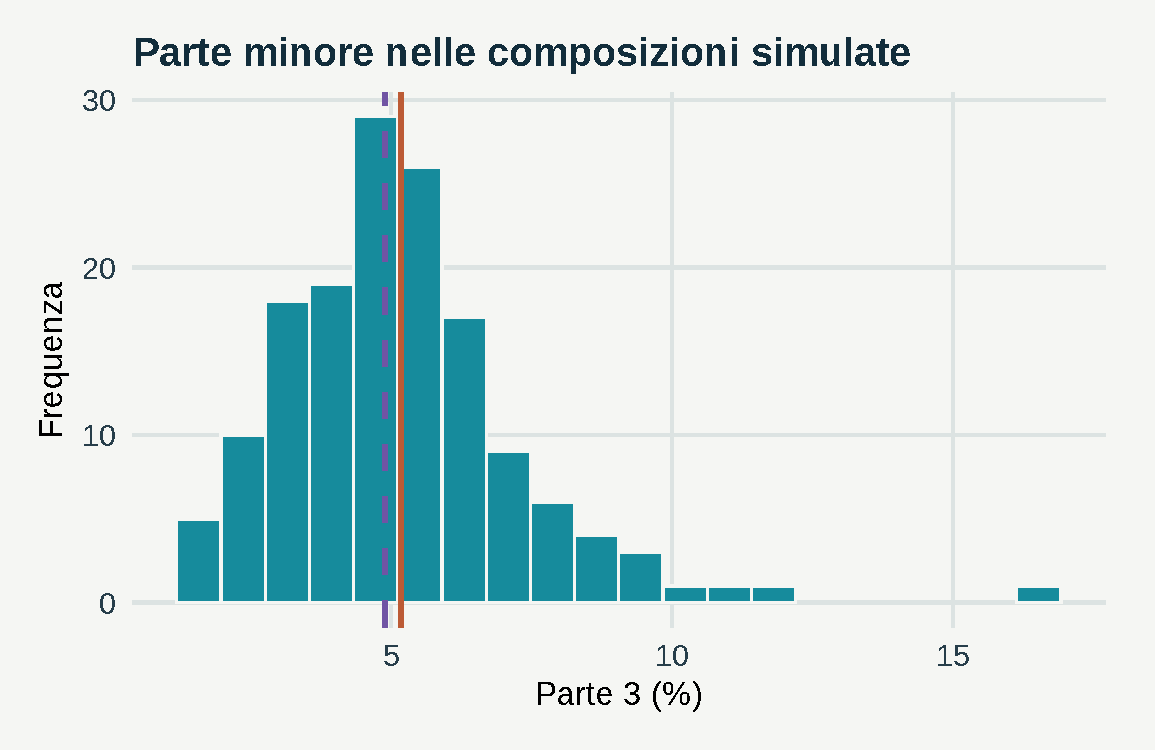
\includegraphics[width=\linewidth,height=6.0cm,keepaspectratio]{Esperimenti/m17-centro-A.pdf}\par}
\PSmall{Deviazione standard dei logaritmi: 0,3. Seme: 17.}
}};
\node[anchor=north west,inner sep=0] at([xshift=10.85cm,yshift=-2.12cm]current page.north west){\Colonna{8.16cm}{\PLabel{Scenario A · simulazione}
\PBody{Il generatore produce centocinquanta composizioni a tre parti attorno al centro (80, 15, 5), con errori gaussiani sui logaritmi delle parti. L’istogramma riporta la parte minore con la media aritmetica, linea continua, e il centro geometrico chiuso, linea tratteggiata.}
\par\smallskip{\centering\adjustbox{max width=.98\linewidth}{$\displaystyle \operatorname{cen}(X)=\mathcal C\Big[\exp\Big(\tfrac1n\sum_k\log x_{k1}\Big),\ldots,\exp\Big(\tfrac1n\sum_k\log x_{kD}\Big)\Big]$}\par\smallskip}
\PSmall{$\mathcal C$ è la chiusura a cento; il centro del generatore è noto per costruzione.}
}};
\node[anchor=north east,inner sep=0] at([xshift=17.1cm,yshift=-12.04cm]current page.north west){\fontsize{7.7}{9}\selectfont \href{https://marzione00.github.io/Lab_Geo/\#laboratorio/m17-centro}{\color{Classical}\bfseries Apri il laboratorio · m17-centro}};
\end{tikzpicture}\end{frame}

\begin{frame}[plain]\hypertarget{slide23}{}
\bookmark[level=1,page=23]{Confronto | Media e centro composizionale}
\begin{tikzpicture}[remember picture,overlay]
\PilotChrome{Confronto | Media e centro composizionale}{DESCRIVERE UN INSIEME DI COMPOSIZIONI}{23}{La media aritmetica di una parte asimmetrica si allontana dal centro al crescere della dispersione.}
\node[anchor=north west,inner sep=0] at([xshift=.96cm,yshift=-2.12cm]current page.north west){\Colonna{9.40cm}{{\centering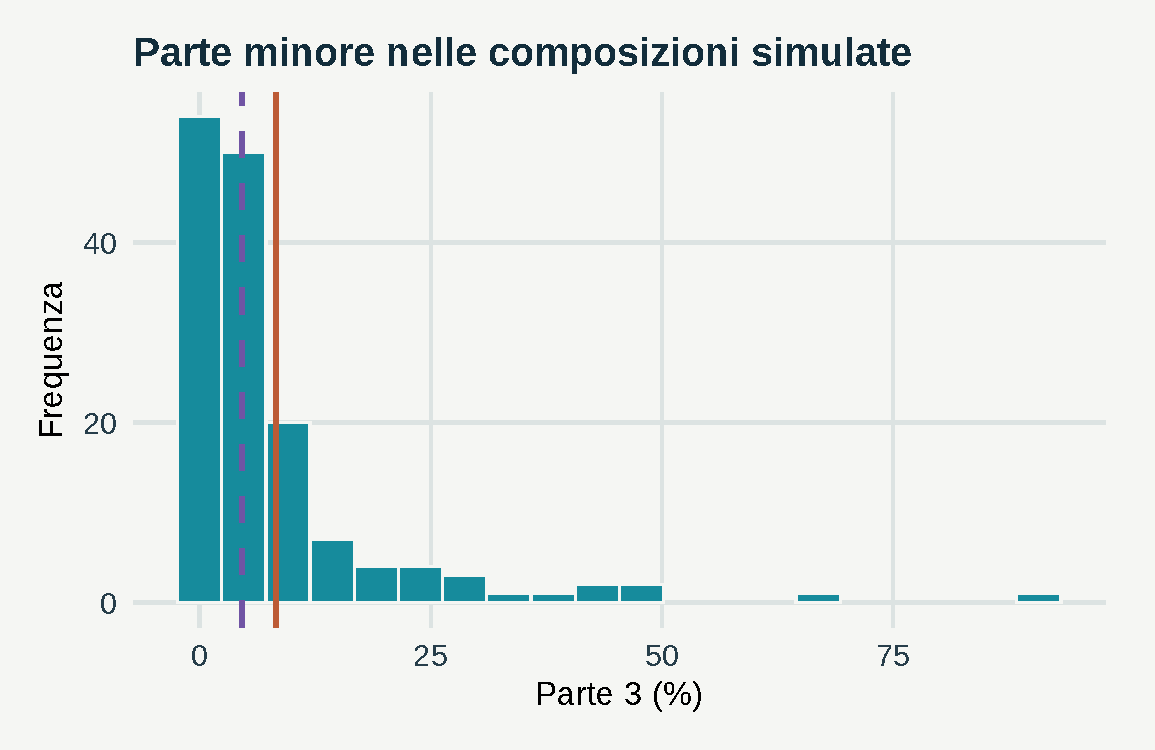
\includegraphics[width=\linewidth,height=5.6cm,keepaspectratio]{Esperimenti/m17-centro-B.pdf}\par}
\PSmall{Deviazione standard dei logaritmi: 0,3 $\to$ 1,2. Tutti gli altri parametri e il seme sono fissi.}
}};
\node[anchor=north west,inner sep=0] at([xshift=10.85cm,yshift=-2.12cm]current page.north west){\Colonna{8.16cm}{\PLabel{Confronto fra gli scenari}
{\fontsize{10.2}{12.8}\selectfont\begin{tabular}{@{}>{\raggedright\arraybackslash}p{0.48\linewidth}@{\hspace{.13cm}}>{\raggedright\arraybackslash}p{0.224\linewidth}@{\hspace{.13cm}}>{\raggedright\arraybackslash}p{0.224\linewidth}@{}}\toprule Grandezza & A & B\\[2.3pt]
\midrule 
Centro del generatore, parte 3 & 5 & 5\\[2.3pt]
Media aritmetica, parte 3 & 5{,}18 & 8{,}25\\[2.3pt]
Centro geometrico, parte 3 & 4{,}89 & 4{,}56\\[2.3pt]
Media aritmetica, parte 1 & 78{,}9 & 69{,}1\\[2.3pt]
Centro geometrico, parte 1 & 80 & 79{,}9\\[2.3pt]
\bottomrule\end{tabular}\par}
\vspace{.25cm}\PBody{Con dispersione 1,2 la media aritmetica della parte minore sale a 8,25\% e quella della parte maggiore scende a 69,1\%; il centro geometrico chiuso resta vicino a (80, 15, 5).}
}};
\node[anchor=north east,inner sep=0] at([xshift=17.1cm,yshift=-12.04cm]current page.north west){\fontsize{7.7}{9}\selectfont \href{https://marzione00.github.io/Lab_Geo/\#laboratorio/m17-centro}{\color{Classical}\bfseries Apri il laboratorio · m17-centro}};
\end{tikzpicture}\end{frame}

\begin{frame}[plain]\hypertarget{slide24}{}
\bookmark[level=0,page=24]{Zeri, limiti di rivelabilità e modelli}
\bookmark[level=1,page=24]{Uno zero impedisce ogni log-rapporto}
\begin{tikzpicture}[remember picture,overlay]
\PilotChrome{Uno zero impedisce ogni log-rapporto}{ZERI, LIMITI DI RIVELABILITÀ E MODELLI}{24}{Prima di trasformare, conta gli zeri e chiarisci da che cosa nascono.}
\node[anchor=north west,inner sep=0] at([xshift=.96cm,yshift=-2.12cm]current page.north west){\Colonna{9.40cm}{\PLabel{Domanda}
\PBody{Quanti campioni hanno una parte registrata come zero, e in quali litologie? Uno zero indica un’assenza o una misura sotto il limite?}
\vspace{.35cm}\PLabel{Interpretazione}
\PBody{Otto arenarie hanno MgO e sette calcari FeO sotto 0,1\%. Le loro somme vanno da 99,90 a 99,95: gli zeri sono valori piccoli non misurati, e la parte esiste.}
}};
\node[anchor=north west,inner sep=0] at([xshift=10.85cm,yshift=-2.12cm]current page.north west){\Colonna{8.16cm}{\begin{tcolorbox}[enhanced,arc=1.7mm,boxrule=.6pt,colback=white,colframe=Classical!60!Navy,colbacktitle=Navy,coltitle=white,fonttitle=\bfseries\small,title={R · calcolo riproducibile},left=1.7mm,right=1.3mm,top=1.1mm,bottom=1.1mm,before skip=1mm,after skip=1.0mm]\lstinputlisting[style=GeoR,language=R]{Codice/capitolo-06.R}\end{tcolorbox}
\PLabel{Risultato in R}
\begin{tcolorbox}[colback=GeoTint,colframe=Rule,boxrule=.5pt,arc=1.4mm,left=2mm,right=1mm,top=1mm,bottom=1mm]{\fontsize{8.6}{11.4}\selectfont\ttfamily \mbox{}\\\mbox{\ \ \ \ \ \ \ \ \ \ \ \ \ \ FeO\ MgO}\\\mbox{\ \ Arenaria\ 40\ \ \ 0\ \ \ 8}\\\mbox{\ \ Basalto\ \ 48\ \ \ 0\ \ \ 0}\\\mbox{\ \ Calcare\ \ 41\ \ \ 7\ \ \ 0}\\\mbox{[1]\ 99.90\ 99.95}}\end{tcolorbox}}};
\end{tikzpicture}\end{frame}

\begin{frame}[plain]\hypertarget{slide25}{}
\bookmark[level=1,page=25]{La sostituzione moltiplicativa}
\begin{tikzpicture}[remember picture,overlay]
\PilotChrome{La sostituzione moltiplicativa}{ZERI, LIMITI DI RIVELABILITÀ E MODELLI}{25}{La sostituzione moltiplicativa conserva i rapporti fra le parti misurate e la somma a cento.}
\node[anchor=north west,inner sep=0] at([xshift=.96cm,yshift=-2.12cm]current page.north west){\Colonna{9.40cm}{\PBody{Josep Antoni Martín-Fernández, Carles Barceló-Vidal e Vera Pawlowsky-Glahn proposero nel 2003 di sostituire gli zeri con un valore $\delta$ e di ridurre le parti misurate dello stesso fattore. Nel codice $\delta$ vale 0,65 volte il limite, una scelta frequente in letteratura; il rapporto SiO$_2$/Al$_2$O$_3$ resta 13,7258 e la somma 100.}
\par\smallskip{\centering\adjustbox{max width=.98\linewidth}{$\displaystyle y_j=\begin{cases}\delta & x_j=0\\[2pt] x_j\Big(1-\dfrac{\sum_{k:x_k=0}\delta}{\kappa}\Big) & x_j>0\end{cases}$}\par\smallskip}
}};
\node[anchor=north west,inner sep=0] at([xshift=10.85cm,yshift=-2.12cm]current page.north west){\Colonna{8.16cm}{\begin{tcolorbox}[enhanced,arc=1.7mm,boxrule=.6pt,colback=white,colframe=Classical!60!Navy,colbacktitle=Navy,coltitle=white,fonttitle=\bfseries\small,title={R · calcolo riproducibile},left=1.7mm,right=1.3mm,top=1.1mm,bottom=1.1mm,before skip=1mm,after skip=1.0mm]\lstinputlisting[style=GeoR,language=R]{Codice/capitolo-07.R}\end{tcolorbox}
\PLabel{Risultato in R}
\begin{tcolorbox}[colback=GeoTint,colframe=Rule,boxrule=.5pt,arc=1.4mm,left=2mm,right=1mm,top=1mm,bottom=1mm]{\fontsize{8.6}{11.4}\selectfont\ttfamily \mbox{\ \ \ somma\ \ \ \ prima\ \ \ \ \ dopo}\\\mbox{100.0000\ \ 13.7258\ \ 13.7258}}\end{tcolorbox}}};
\end{tikzpicture}\end{frame}

\begin{frame}[plain]\hypertarget{slide26}{}
\bookmark[level=1,page=26]{Il valore sostitutivo sposta i risultati}
\begin{tikzpicture}[remember picture,overlay]
\PilotChrome{Il valore sostitutivo sposta i risultati}{ZERI, LIMITI DI RIVELABILITÀ E MODELLI}{26}{Un risultato che dipende dagli zeri si riporta con la sua sensibilità al valore sostitutivo.}
\node[anchor=north west,inner sep=0] at([xshift=.96cm,yshift=-2.12cm]current page.north west){\Colonna{9.40cm}{{\centering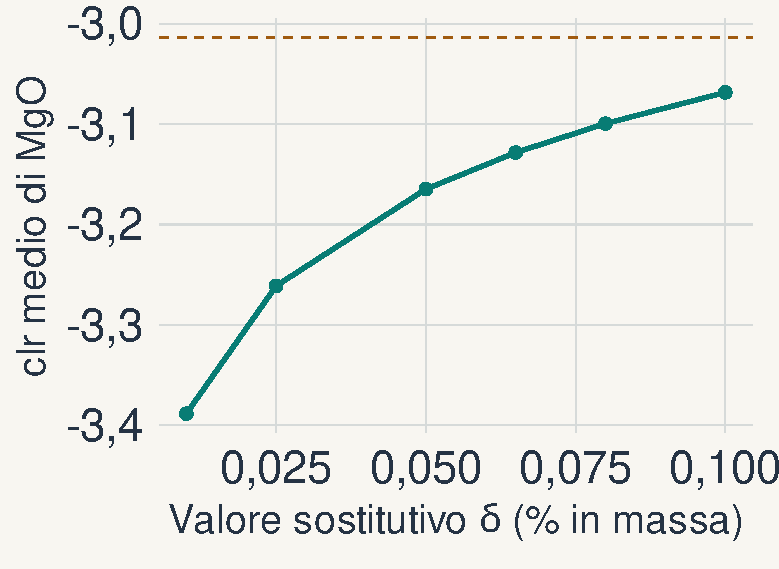
\includegraphics[width=\linewidth,height=6.15cm,keepaspectratio]{Figure/F06.pdf}\par}
\PSmall{Media della coordinata clr di MgO nelle 48 arenarie al variare di $\delta$; la linea tratteggiata usa le sole 40 arenarie senza zeri.}
}};
\node[anchor=north west,inner sep=0] at([xshift=10.85cm,yshift=-2.12cm]current page.north west){\Colonna{8.16cm}{\PBody{Nelle arenarie la media della coordinata clr di MgO vale $-3{,}39$ con $\delta=0{,}01$, $-3{,}13$ con $\delta=0{,}065$ e $-3{,}07$ con $\delta=0{,}1$. Escludere gli otto campioni con lo zero dà $-3{,}01$, un valore più alto perché elimina proprio le arenarie più povere di magnesio.}
\PSmall{$\delta$ è espresso in percentuale in massa; il limite di rivelabilità è 0,1\%.}
}};
\end{tikzpicture}\end{frame}

\begin{frame}[plain]\hypertarget{slide27}{}
\bookmark[level=1,page=27]{Una composizione come predittore}
\begin{tikzpicture}[remember picture,overlay]
\PilotChrome{Una composizione come predittore}{ZERI, LIMITI DI RIVELABILITÀ E MODELLI}{27}{In un modello lineare le parti di una composizione entrano attraverso $D-1$ coordinate.}
\node[anchor=north west,inner sep=0] at([xshift=.96cm,yshift=-2.12cm]current page.north west){\Colonna{9.40cm}{{\centering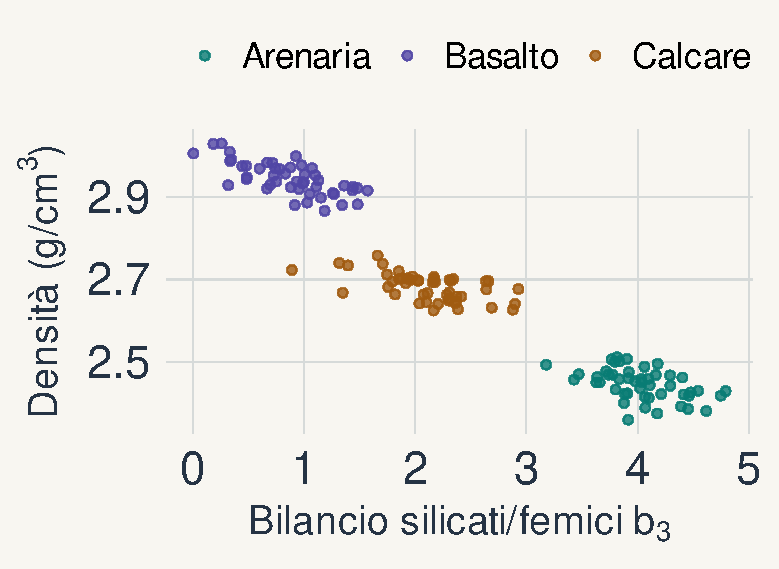
\includegraphics[width=\linewidth,height=6.15cm,keepaspectratio]{Figure/F03.pdf}\par}
\PSmall{Densità e bilancio $b_3$ fra SiO$_2$, Al$_2$O$_3$ e MgO, FeO, per litologia.}
}};
\node[anchor=north west,inner sep=0] at([xshift=10.85cm,yshift=-2.12cm]current page.north west){\Colonna{8.16cm}{\PBody{Le sei percentuali non possono entrare insieme in una regressione, perché la loro somma è costante. I cinque bilanci della partizione sono coordinate libere: il modello della densità con i bilanci spiega il 97,3\% della varianza, quello con cinque percentuali il 94,8\%. Il bilancio $b_3$ confronta silicati e ossidi femici.}
\par\smallskip{\centering\adjustbox{max width=.98\linewidth}{$\displaystyle b_3=\log\frac{(x_{\mathrm{SiO_2}}x_{\mathrm{Al_2O_3}})^{1/2}}{(x_{\mathrm{MgO}}x_{\mathrm{FeO}})^{1/2}}$}\par\smallskip}
}};
\end{tikzpicture}\end{frame}

\begin{frame}[plain]\hypertarget{slide28}{}
\bookmark[level=1,page=28]{Interpretare un coefficiente di bilancio}
\begin{tikzpicture}[remember picture,overlay]
\PilotChrome{Interpretare un coefficiente di bilancio}{ZERI, LIMITI DI RIVELABILITÀ E MODELLI}{28}{Un coefficiente di bilancio descrive l’effetto di un cambiamento relativo fra due gruppi di parti.}
\node[anchor=north west,inner sep=0] at([xshift=.96cm,yshift=-2.12cm]current page.north west){\Colonna{9.40cm}{\PBody{Il codice stima la densità con il bilancio $b_3$ e la litologia. A parità di litologia, un aumento unitario di $b_3$ moltiplica per $e\approx2{,}72$ il rapporto fra la media geometrica di silice e allumina e quella degli ossidi femici, e corrisponde a una densità più bassa di 0,057 g/cm$^3$.}
\par\smallskip{\centering\adjustbox{max width=.98\linewidth}{$\displaystyle \rho=\beta_0+\beta_1 b_3+\gamma_{\mathrm{Bas}}+\gamma_{\mathrm{Cal}}+\varepsilon$}\par\smallskip}
}};
\node[anchor=north west,inner sep=0] at([xshift=10.85cm,yshift=-2.12cm]current page.north west){\Colonna{8.16cm}{\begin{tcolorbox}[enhanced,arc=1.7mm,boxrule=.6pt,colback=white,colframe=Classical!60!Navy,colbacktitle=Navy,coltitle=white,fonttitle=\bfseries\small,title={R · calcolo riproducibile},left=1.7mm,right=1.3mm,top=1.1mm,bottom=1.1mm,before skip=1mm,after skip=1.0mm]\lstinputlisting[style=GeoR,language=R]{Codice/capitolo-08.R}\end{tcolorbox}
\PLabel{Risultato in R}
\begin{tcolorbox}[colback=GeoTint,colframe=Rule,boxrule=.5pt,arc=1.4mm,left=2mm,right=1mm,top=1mm,bottom=1mm]{\fontsize{8.6}{11.4}\selectfont\ttfamily \mbox{intercetta\ \ \ \ \ \ \ \ \ b3\ \ \ \ \ \ \ Bas.\ \ \ \ \ \ \ Cal.}\\\mbox{\ \ \ \ \ 2.676\ \ \ \ \ -0.057\ \ \ \ \ \ 0.318\ \ \ \ \ \ 0.126}}\end{tcolorbox}}};
\end{tikzpicture}\end{frame}

\begin{frame}[plain]\hypertarget{slide29}{}
\bookmark[level=1,page=29]{Valori sotto il limite e sostituzione}
\begin{tikzpicture}[remember picture,overlay]
\PilotChrome{Valori sotto il limite e sostituzione}{ZERI, LIMITI DI RIVELABILITÀ E MODELLI}{29}{Valutare come la sostituzione dei valori sotto il limite sposta la media di un log-rapporto.}
\node[anchor=north west,inner sep=0] at([xshift=.96cm,yshift=-2.12cm]current page.north west){\Colonna{9.40cm}{{\centering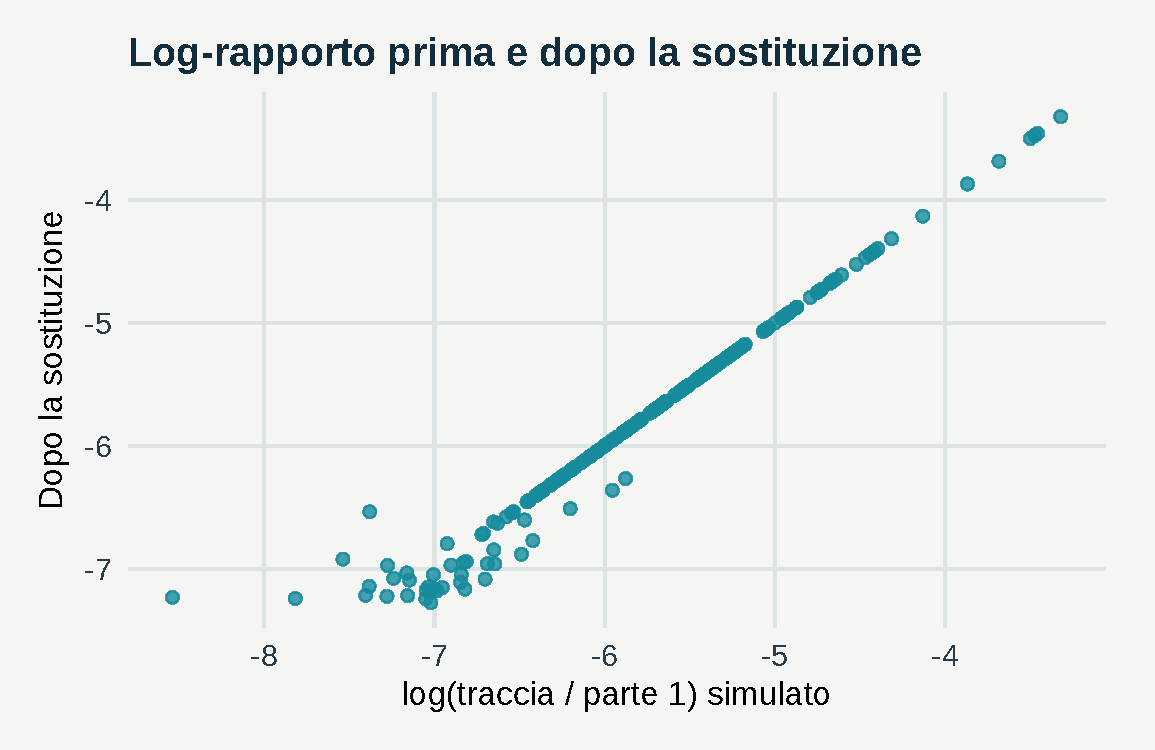
\includegraphics[width=\linewidth,height=6.0cm,keepaspectratio]{Esperimenti/m17-zeri-A.pdf}\par}
\PSmall{Limite di rivelabilità: 0,1\%; valore sostitutivo 0,65 volte il limite. Seme: 17.}
}};
\node[anchor=north west,inner sep=0] at([xshift=10.85cm,yshift=-2.12cm]current page.north west){\Colonna{8.16cm}{\PLabel{Scenario A · simulazione}
\PBody{Il generatore produce duecento composizioni a quattro parti con una traccia di mediana 0,2\%. Le misure della traccia sotto il limite diventano zero e vengono sostituite in modo moltiplicativo; il grafico confronta il log-rapporto simulato con quello dopo la sostituzione.}
\par\smallskip{\centering\adjustbox{max width=.98\linewidth}{$\displaystyle \bar\ell=\frac1n\sum_{k=1}^n\log\frac{y_{k4}}{y_{k1}}$}\par\smallskip}
\PSmall{$y_{k4}$ è la traccia del campione $k$ dopo la sostituzione e $y_{k1}$ la parte maggiore.}
}};
\node[anchor=north east,inner sep=0] at([xshift=17.1cm,yshift=-12.04cm]current page.north west){\fontsize{7.7}{9}\selectfont \href{https://marzione00.github.io/Lab_Geo/\#laboratorio/m17-zeri}{\color{Classical}\bfseries Apri il laboratorio · m17-zeri}};
\end{tikzpicture}\end{frame}

\begin{frame}[plain]\hypertarget{slide30}{}
\bookmark[level=1,page=30]{Confronto | Valori sotto il limite e sostituzione}
\begin{tikzpicture}[remember picture,overlay]
\PilotChrome{Confronto | Valori sotto il limite e sostituzione}{ZERI, LIMITI DI RIVELABILITÀ E MODELLI}{30}{La media dopo la sostituzione dipende dal valore scelto e dalla quota di campioni sotto il limite.}
\node[anchor=north west,inner sep=0] at([xshift=.96cm,yshift=-2.12cm]current page.north west){\Colonna{9.40cm}{{\centering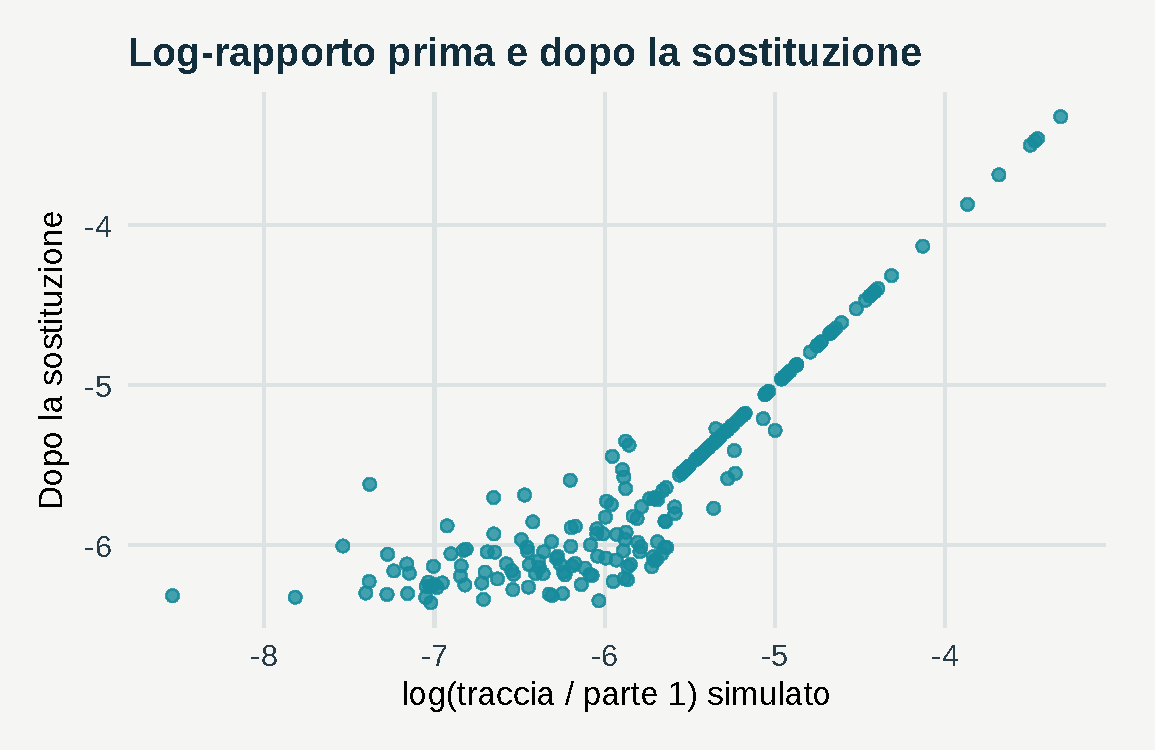
\includegraphics[width=\linewidth,height=5.6cm,keepaspectratio]{Esperimenti/m17-zeri-B.pdf}\par}
\PSmall{Limite di rivelabilità: 0,1 $\to$ 0,25\%. Tutti gli altri parametri e il seme sono fissi.}
}};
\node[anchor=north west,inner sep=0] at([xshift=10.85cm,yshift=-2.12cm]current page.north west){\Colonna{8.16cm}{\PLabel{Confronto fra gli scenari}
{\fontsize{10.2}{12.8}\selectfont\begin{tabular}{@{}>{\raggedright\arraybackslash}p{0.48\linewidth}@{\hspace{.13cm}}>{\raggedright\arraybackslash}p{0.224\linewidth}@{\hspace{.13cm}}>{\raggedright\arraybackslash}p{0.224\linewidth}@{}}\toprule Grandezza & A & B\\[2.3pt]
\midrule 
Quota sotto il limite & 0{,}195 & 0{,}62\\[2.3pt]
Media simulata & -5{,}79 & -5{,}79\\[2.3pt]
Media con sostituzione & -5{,}79 & -5{,}61\\[2.3pt]
Media escludendo i campioni & -5{,}5 & -4{,}96\\[2.3pt]
\bottomrule\end{tabular}\par}
\vspace{.25cm}\PBody{Con il limite a 0,25\% il 62\% dei campioni è sotto il limite. La sostituzione sposta la media da $-5{,}79$ a $-5{,}61$; escludere i campioni la porta a $-4{,}96$.}
}};
\node[anchor=north east,inner sep=0] at([xshift=17.1cm,yshift=-12.04cm]current page.north west){\fontsize{7.7}{9}\selectfont \href{https://marzione00.github.io/Lab_Geo/\#laboratorio/m17-zeri}{\color{Classical}\bfseries Apri il laboratorio · m17-zeri}};
\end{tikzpicture}\end{frame}

\begin{frame}[plain]\hypertarget{slide31}{}
\bookmark[level=0,page=31]{Sintesi}
\bookmark[level=1,page=31]{Dal risultato alla relazione}
\begin{tikzpicture}[remember picture,overlay]
\PilotChrome{Dal risultato alla relazione}{SINTESI}{31}{Riporta i log-rapporti usati, il trattamento degli zeri e la sensibilità dei risultati.}
\node[anchor=north west,inner sep=0] at([xshift=.96cm,yshift=-2.12cm]current page.north west){\Colonna{9.40cm}{\PLabel{Domanda di partenza}
\PBody{La correlazione di −0,92 fra SiO$_2$ e CaO descrive la geochimica o la somma a cento?}
\PLabel{Risultato da discutere}
\PBody{La correlazione di $-0{,}92$ fra SiO$_2$ e CaO nasce soprattutto dal confronto fra arenarie e calcari e dal vincolo della somma: nei basalti vale 0,07. I log-rapporti descrivono le relazioni fra le parti senza dipendere dalla chiusura, e la densità dipende dal bilancio fra silicati e ossidi femici.}
}};
\node[anchor=north west,inner sep=0] at([xshift=10.85cm,yshift=-2.12cm]current page.north west){\Colonna{8.16cm}{\PLabel{Limiti della conclusione}
\PBody{I campioni sono sintetici, generati con errori indipendenti sui logaritmi. Le quindici misure sotto il limite sono sostituite con un valore convenzionale, e le stime che le coinvolgono vanno lette con la loro sensibilità a $\delta$.}
\vspace{.4cm}\href{https://marzione00.github.io/Lab_Geo/\#modulo-M17}{\color{Classical}\bfseries Torna agli esperimenti di Simplex}
}};
\end{tikzpicture}\end{frame}

\begin{frame}[plain]\hypertarget{slide32}{}
\bookmark[level=0,page=32]{Riferimenti}
\bookmark[level=1,page=32]{Fonti, dati e codice per riprodurre le figure}
\begin{tikzpicture}[remember picture,overlay]
\PilotChrome{Fonti, dati e codice per riprodurre le figure}{RIFERIMENTI}{32}{I risultati numerici si riferiscono ai dati e alle ipotesi dichiarate nel caso.}
\node[anchor=north west,inner sep=0] at([xshift=.96cm,yshift=-2.12cm]current page.north west){\Colonna{9.40cm}{\PLabel{Fonti}
{\fontsize{9.4}{12.2}\selectfont K. Pearson, Proceedings of the Royal Society of London 60, 489–498, 1897.\par F. Chayes, Journal of Geophysical Research 65(12), 4185–4193, 1960.\par J. Aitchison, Journal of the Royal Statistical Society B 44(2), 139–160, 1982.\par J. Aitchison e M. Greenacre, Applied Statistics 51(4), 375–392, 2002.\par J. J. Egozcue e colleghi, Mathematical Geology 35(3), 279–300, 2003.\par J. J. Egozcue e V. Pawlowsky-Glahn, Mathematical Geology 37(7), 795–828, 2005.\par J. A. Martín-Fernández, C. Barceló-Vidal e V. Pawlowsky-Glahn, Mathematical Geology 35(3), 253–278, 2003.\par}
}};
\node[anchor=north west,inner sep=0] at([xshift=10.85cm,yshift=-2.12cm]current page.north west){\Colonna{8.16cm}{\PLabel{Dati e codice}
\PBody{Dati sintetici del corso (composizioni\_v1.csv), generati da R/genera\_dati.R. Codice contiene i frammenti delle pagine; R/M17\_figure.R ricostruisce figure e valori; Esperimenti contiene i programmi dei due scenari e Diagrammi i disegni TikZ.}
\vspace{.3cm}\href{https://marzione00.github.io/Lab_Geo/\#lezione-M17}{\color{Classical}\bfseries Apri le tappe di Simplex su GeoStat Lab}
}};
\end{tikzpicture}\end{frame}
\end{document}
